% ============================================================
% Master rad , Primena veštačke inteligencije u obrazovanju:
%              veliki jezički modeli za testiranje i ocenjivanje
%              studenata
% (naslov je usklađen sa naslovom u prijavi rada)
% Autor: Svetozar Iković, Matematički fakultet, UB
%
% Zvanični šablon MATF-a: paket matfmaster (Filip Marić, 2015),
% preuzet sa https://www.matf.bg.ac.rs/nastava/master-radovi/
% (teze.zip). Uz njega idu matfmaster.sty, hyperref.cfg,
% serbian*.lbx/ldf i matf.png u ovom direktorijumu.
% Kompajliranje: tectonic main.tex (XeTeX). Potrebni su fontovi
% CMU Serif i Open Sans (u teze.zip/fonts; na Ubuntu paketi
% fonts-cmu i fonts-open-sans, na macOS kopirati u ~/Library/Fonts).
% ============================================================
\documentclass[12pt,oneside]{memoir}

% Paket koji definiše sve specifičnosti master rada Matematičkog fakulteta
% (naslovna strana, strana komisije, rezime, zaglavlja, margine, fontovi, jezik).
\usepackage[latinica]{matfmaster}

% --- Matematika, tabele ---
\usepackage{amsmath}
\usepackage{booktabs}
\usepackage{makecell}
\usepackage{multirow}

% --- Prompt kutije (kao u ComSIS radu) ---
\usepackage[most]{tcolorbox}
\usepackage{enumitem}
\tcbset{
  promptbox/.style={
    colback=gray!3,
    colframe=black,
    boxrule=0.4pt,
    arc=2pt,
    left=6pt, right=6pt, top=6pt, bottom=6pt,
    breakable
  }
}

% --- Dijagram arhitekture ---
\usepackage{tikz}
\usetikzlibrary{arrows.meta, positioning, shapes.geometric}

% --- Kod ---
\usepackage{listings}
\usepackage{xcolor}
\lstset{
  basicstyle=\ttfamily\small,
  breaklines=true,
  frame=single,
  framerule=0.3pt,
  captionpos=b,
  showstringspaces=false
}

% Marker za nedovršene delove , pretragom po \todo lako se
% nalazi šta je preostalo; pre predaje ne sme ostati nijedan.
\newcommand{\todo}[1]{\textcolor{red}{\textbf{[TODO: #1]}}}

% --- Metapodaci rada ---
\bib{literatura}
\autor{Svetozar Iković}
\naslov{Primena veštačke inteligencije u obrazovanju: veliki jezički modeli za testiranje i ocenjivanje studenata}
\godina{2026}
\mentor{prof. dr Jelena \textsc{Graovac}\\ Univerzitet u Beogradu, Matematički fakultet}
\komisijaA{prof. dr Milena \textsc{Vujošević Janičić}\\ Univerzitet u Beogradu, Matematički fakultet}
\komisijaB{prof. dr Saša \textsc{Malkov}\\ Univerzitet u Beogradu, Matematički fakultet}
% \datumodbrane{...}  % ako se ne navede, ostaje crta za ručni upis
\section*{Zahvalnica}
Zahvaljujem se...

\newpage

\section*{Rezime}

Ubrzani razvoj veštačke inteligencije i velikih jezičkih modela (engl.
\emph{large language models}, LLM) menja praksu provere znanja u visokom obrazovanju,
naročito u ocenjivanju pitanja otvorenog tipa.
Tradicionalno ocenjivanje je vremenski zahtevno, sklono nedoslednosti i teško skalabilno za velike grupe studenata.
Veliki jezički modeli tumače slobodan tekst i rezonuju o njegovom značenju,
pa povratna informacija može biti brža, doslednija i češća.
U ovom radu predstavljen je EduGrader, platforma za ocenjivanje otvorenog koda koja objedinjuje GPT-4o,
GPT-4o-mini, DeepSeek-Chat, GPT-5 i DeepSeek-Reasoner.
EduGrader podržava tri konfiguracije strogosti ocenjivanja (blagu, neutralnu,
strogu) i uz numeričku ocenu daje sažeto obrazloženje: šta je u odgovoru ispravno, šta nedostaje i gde je greška.
Sistem radi u dva režima: režimu sa zadatim referentnim odgovorom (engl. \emph{provided-reference-answer}, PRA),
vođenom referentnim odgovorima nastavnika,
i režimu sa generisanim referentnim odgovorom (engl. \emph{generated-reference-answer}, GRA),
koji referentne odgovore automatski konstruiše iz nastavnih materijala.
Svi eksperimenti sprovedeni su na srpskom, jeziku sa ograničenim resursima koji je slabo zastupljen u podacima za obučavanje savremenih modela,
dakle izvan engleskog konteksta u kome se ovakvi sistemi obično ispituju.
EduGrader je evaluiran na 583 autentična studentska odgovora sa pet univerzitetskih kurseva na dve institucije,
uključujući tekstualna objašnjenja i odgovore u obliku koda.
U najboljoj konfiguraciji sistem postiže Pirsonov koeficijent korelacije od 0{,}89 sa ljudskim ocenjivačima.
Zamišljen je kao pomoć nastavniku koja preuzima rutinski deo ocenjivanja, a ne kao njegova zamena.

\vspace{1em}
\noindent\textbf{Ključne reči:} veliki jezički modeli, automatsko ocenjivanje, pitanja otvorenog tipa, referentni odgovor,
srpski jezik, jezik sa ograničenim resursima, procena znanja u visokom obrazovanju, EduGrader.
\newpage
   % \apstr{...} i \kljucnereci{...}

\begin{document}

% ------------------------------------------------------------
% Uvodne strane: naslovna, komisija, zahvalnica, rezime, sadržaj
% ------------------------------------------------------------
\frontmatter
\naslovna
\komisija
% Zahvalnica (posebna strana pre rezimea)
\chapter*{Zahvalnica}
\thispagestyle{empty}
Zahvaljujem se mentorki, prof. dr Jeleni Graovac, na pomoći i podršci tokom celokupne izrade ovog rada,
od početne ideje do realizacije, na usmeravanju istraživanja i na strpljivom čitanju svake verzije teksta teze.

\apstrakt
\tableofcontents*

% ------------------------------------------------------------
% Poglavlja
% ------------------------------------------------------------
\mainmatter
% 1. Uvod
\section{Uvod}
\label{sec:uvod}

Ocenjivanje retko predstavlja najzanimljiviji deo nastave, ali oblikuje način na koji studenti uče.
Pravovremena i konkretna povratna informacija pomaže studentu da ispravi nesporazum pre nego što se ustali;
kada kasni ili je neodređena, provera znanja postaje formalnost.
Na velikim univerzitetskim kursevima nastavnici i saradnici moraju da ocene stotine odgovora otvorenog tipa u kratkim rokovima.
Kratka objašnjenja i mini-eseji, za razliku od pitanja sa ponuđenim odgovorima, ne mogu se proveriti prostim uparivanjem obrazaca.
Oni zahtevaju tumačenje: prepoznavanje delimično ispravnog rezonovanja,
razlikovanje jezičkih nepreciznosti od konceptualnih praznina i odluku o tome koliko neki propust treba da utiče na ocenu.
Takvo ocenjivanje je skupo, teško primenljivo na velike grupe studenata i sklono nedoslednosti:
čak i uz detaljna uputstva, dva ocenjivača mogu isti odgovor protumačiti različito,
naročito kada je odgovor dvosmislen, pisan u žurbi ili strukturno nejasan~\cite{brookhart2016century,jonsson2007use,stemler2004comparison}.
Nastavnika to opterećenje odvraća od pitanja zasnovanih na objašnjenjima,
a student povratnu informaciju dobija prekasno da bi mu koristila, ili je ne dobija uopšte.

Ranije generacije sistema za automatsku proveru znanja funkcionisale su samo kada su odgovori bili strogo ograničeni:
testovi sa ponuđenim odgovorima,
pitanja dopunjavanja ili kratki odgovori sa predvidljivom formulacijom~\cite{brew2013automated,ramesh2022automated,shermis2003automated}.
Napredak u obradi prirodnog jezika proširio je ove mogućnosti, ali su se mnogi pristupi i dalje oslanjali na ručno projektovanje atributa,
uske domene ili velike označene skupove podataka~\cite{banko2001scaling,collobert2008unified,sebastiani2002machine}.
Savremeni veliki jezički modeli (engl. \emph{large language models}, LLM) mogu da analiziraju i tumače odgovore formulisane slobodnim tekstom.
Time je postalo izvodljivo projektovati alate koji ocenjuju odgovore otvorenog tipa,
obrazlažu ocenu prirodnim jezikom i ukazuju na ono što u odgovoru nedostaje,
a ne samo na ono što je pogrešno~\cite{kasneci2023chatgpt,zhai2023chatgpt}.

\subsection{Motivacija}
\label{sec:motivacija}

Cilj ovog rada je ispitivanje mogućnosti pouzdane primene velikih jezičkih modela kao podrške u ocenjivanju.
Ručno ocenjivanje troši veliki deo nastavničkog vremena, pa povratna informacija kasni,
a provere znanja se organizuju ređe nego što bi bilo korisno.
Automatizovan sistem za ocenjivanje menja tu ravnotežu.
Provere znanja mogu biti češće, pa student kontinuirano prati napredak i prepoznaje oblasti koje zahtevaju dodatni rad.
Analiza odgovora stiže dok je gradivo još sveže.
Vreme koje bi otišlo na rutinski deo ocenjivanja nastavnik usmerava na individualnu podršku studentima.

Upotreba velikih jezičkih modela u ocenjivanju istovremeno otvara praktična i pedagoška pitanja.
Ovaj rad razmatra četiri:
\begin{enumerate}
    \item Koliko su ocene velikih jezičkih modela usklađene sa nastavničkim i koliko su dosledne kroz različite predmete i tipove pitanja?
    \item Mogu li nastavnici kalibrisati strogost ocenjivanja prema očekivanjima konkretnog kursa?
    \item Šta se dešava kada potpun referentni odgovor nastavnika nije dostupan?
    \item Kako sistem za automatizovano ocenjivanje projektovati tako da nastavnik zadrži kontrolu nad konačnom ocenom?
\end{enumerate}
Na ova pitanja rad se vraća u zaključku (poglavlje~\ref{sec:zakljucak}).

\subsection{Sistem EduGrader i doprinosi rada}

U ovom radu predstavljen je EduGrader, platforma za ocenjivanje pitanja otvorenog tipa u visokom obrazovanju, pod nadzorom nastavnika.
EduGrader objedinjuje više velikih jezičkih modela,
GPT-4o,\footnote{\url{https://platform.openai.com/docs/models/gpt-4o}}
GPT-4o-mini,\footnote{\url{https://platform.openai.com/docs/models/gpt-4o-mini}}
DeepSeek-Chat,\footnote{\url{https://api-docs.deepseek.com/}} i dva modela za rezonovanje (engl. \emph{reasoning models}),
GPT-5\footnote{\url{https://platform.openai.com/docs/models/gpt-5}}
i DeepSeek-Reasoner,\footnote{\url{https://api-docs.deepseek.com/guides/reasoning\_model}}
u jedinstven tok ocenjivanja u kome poslednju reč ima nastavnik.
Sistem podržava tri konfiguracije strogosti ocenjivanja: blagu, neutralnu i strogu.
Podela odgovara nastavnoj praksi, u kojoj neki kursevi nagrađuju delimično ispravno rezonovanje,
dok drugi zahtevaju preciznu terminologiju i potpuna rešenja.

EduGrader nudi dva komplementarna režima ocenjivanja:
\begin{itemize}
    \item \textbf{Režim sa zadatim referentnim odgovorom} (engl. \emph{provided-reference-answer}, PRA),
    u kome se studentski odgovori porede sa referentnim odgovorima koje je pripremio nastavnik.
    \item \textbf{Režim sa generisanim referentnim odgovorom} (engl. \emph{generated-reference-answer}, GRA),
    u kome sistem najpre generiše referentni odgovor na osnovu nastavnih materijala,
    beležaka sa predavanja, skripti i udžbenika,
    a zatim studentske odgovore ocenjuje u odnosu na tako generisani standard.
\end{itemize}

Izlaz u oba režima je numerička ocena praćena obrazloženjem koje ukazuje na jake strane odgovora, koncepte koji nedostaju i praznine u rezonovanju.
Takva povratna informacija studentu je upotrebljiva, a nastavniku proverljiva, za razliku od ocene koja dolazi iz „crne kutije''.

Model ocenu izražava na skali od 0 do 100, jer finija granulacija olakšava razlikovanje bliskih nivoa kvaliteta odgovora.
Dobijena vrednost se zatim preslikava na skalu od 0 do 10, na kojoj ocenjuju nastavnici (detalji u odeljku~\ref{sec:pipeline}).
Sve ocene u ovom radu, i sistemske i nastavničke, prikazane su na skali 0--10, osim tamo gde je naznačeno drugačije.

Svi eksperimenti sprovedeni su na srpskom jeziku,
koji spada u jezike sa ograničenim resursima i znatno je manje zastupljen u podacima za obučavanje savremenih modela,
čime je ispitivanje prošireno izvan dominantnog engleskog jezičkog konteksta.
Sistem je evaluiran na 583 autentična studentska odgovora prikupljena na dva univerziteta i pet kurseva,
od kratkih činjeničkih odgovora i otvorenih tekstualnih objašnjenja do odgovora u obliku koda.
Rezultati pokazuju da PRA režim daje stabilnije ishode od GRA režima i da modeli za rezonovanje daju ocene najbliže nastavničkim.
U najboljoj konfiguraciji (GPT-5, blaga strogost) EduGrader postiže Pirsonov koeficijent korelacije (engl.
\emph{Pearson correlation coefficient}, PCC) od 0{,}89 u odnosu na ljudsko ocenjivanje, a u neutralnoj konfiguraciji 0{,}88.

EduGrader je zamišljen kao alat za podršku ocenjivanju, a ne kao zamena za nastavnika.
Namenjen je smanjenju repetitivnog dela ocenjivanja,
ali ljudski nadzor ostaje neophodan za dvosmislena pitanja, očekivanja specifična za disciplinu i granične slučajeve.
Zato je sistem projektovan po principu čoveka u petlji (engl.
\emph{human-in-the-loop}) i objavljen kao softver otvorenog koda\footnote{\url{https://github.com/toswe/Master}},
kako bi bio proverljiv i prilagodljiv drugim institucijama.
Postupak ponovnog izvođenja svih prikazanih rezultata opisan je u odeljku~\ref{sec:reprodukcija}.

Doprinosi rada su sledeći:
\begin{enumerate}
    \item \textbf{Veb aplikacija EduGrader} (poglavlje~\ref{sec:aplikacija}):
    nastavnički i studentski modul, serverski modul za ocenjivanje koji čuva prompt, odgovor modela i izdvojenu ocenu za svaki ocenjeni odgovor,
    i integracioni sloj koji više provajdera jezičkih modela pokriva jednim interfejsom.
    \item \textbf{Sistem za automatizovanu evaluaciju modela} (poglavlje~\ref{sec:pipeline}):
    reproducibilan \emph{pipeline} koji nad ručno pripremljenim ispitnim podacima pokreće ocenjivanje
    za proizvoljnu kombinaciju modela, konfiguracije strogosti i režima i računa metrike korelacije i slaganja sa ocenama nastavnika.
    \item \textbf{Skup podataka na srpskom jeziku}: 583 autentična, pseudonimizovana studentska odgovora sa pet kurseva na dve institucije,
    sa nastavničkim ocenama i referentnim odgovorima (odeljci~\ref{sec:podaci} i~\ref{sec:etika}).
    \item \textbf{Sistematska evaluacija}: pet modela u tri konfiguracije strogosti i dva režima ocenjivanja,
    dopunjena eksperimentima sa nastavnim materijalom u promptu i sa temperaturom (poglavlje~\ref{sec:rezultati}).
    \item \textbf{Empirijski nalazi}: referentni odgovor nastavnika dosledno poboljšava i korelaciju i slaganje sa ljudskim ocenjivačima,
    modeli za rezonovanje su im najbliži, a stroga konfiguracija po pravilu pogoršava oba;
    najbolja konfiguracija dostiže PCC od 0{,}89.
\end{enumerate}

\subsection{Struktura rada}

Poglavlje~\ref{sec:pregled} daje pregled srodnih istraživanja primene veštačke inteligencije u ocenjivanju
i pozicionira ovaj rad u odnosu na njih.
Poglavlje~\ref{sec:aplikacija} opisuje veb aplikaciju EduGrader i sloj za integraciju jezičkih modela,
a poglavlje~\ref{sec:pipeline} sistem za automatizovanu evaluaciju modela kojim su sprovedeni eksperimenti.
Poglavlje~\ref{sec:metodologija} predstavlja metodologiju evaluacije: metrike, skupove podataka, zaštitu podataka i konfiguracije modela.
Poglavlje~\ref{sec:rezultati} donosi rezultate, uključujući poređenje PRA i GRA režima kroz modele i konfiguracije strogosti,
uticaj konfiguracije strogosti i korelacije po pojedinačnim kursevima.
U poglavlju~\ref{sec:diskusija} rezultati su upoređeni sa prethodnim istraživanjima i razmotreni su pravci budućeg rada,
dok poglavlje~\ref{sec:zakljucak} zaključuje rad.
Dodatak~\ref{app:promptovi} sadrži šablone promptova (engl. \emph{prompt}) i reprezentativne primere ocenjivanja.

% 2. Pregled oblasti i srodni radovi
\section{Pregled oblasti i srodni radovi}
\label{sec:pregled}

Primena veštačke inteligencije u obrazovanju razvijala se od rane automatizacije zasnovane na pravilima ka adaptivnim sistemima koji tumače i generišu složene odgovore nalik ljudskim.
Pod veštačkom inteligencijom se podrazumevaju računarski sistemi projektovani da obavljaju kognitivne funkcije poput učenja, rezonovanja i rešavanja problema~\cite{baker2019educ},
a u obrazovnom kontekstu skup tehnologija koje omogućavaju personalizovanija i adaptivnija okruženja za učenje~\cite{zawacki2019systematic}.
Sistematski pregledi im pripisuju potencijal da unaprede ishode učenja, prošire dostupnost obrazovanja i efikasnije iskoriste nastavne resurse~\cite{yuskovych2022application,zhang2023study}.
Veliki jezički modeli tu donose promenu u odnosu na ranije pristupe zasnovane na obradi prirodnog jezika:
ne zahtevaju ručno projektovane atribute ni obučavanje za konkretan domen,
već obrađuju slobodan tekst i rezonuju o značenju na višem nivou apstrakcije.
Zato se ispituju za nastavu usmerenu na učenika, automatsko generisanje sadržaja i nove oblike provere znanja~\cite{zhang2023study}.

Empirijske studije ocenjivanja uz podršku velikih jezičkih modela daju mešovite rezultate.
Kuli i Jusuf~\cite{kooli2025transforming} ispitali su ocenjivanje uz pomoć ChatGPT-a na 25 studentskih radova iz kohorte od približno 100 studenata druge godine na kursu iz društvenih nauka,
gde su radove nezavisno ocenili i ljudski ocenjivači i model.
Dobijena je umerena korelacija između ocena veštačke inteligencije i ljudskih ocena (koeficijent korelacije približno 0{,}45): model aproksimira opšte obrasce ocenjivanja,
ali pojedinačne evaluacije se i dalje razlikuju.
Autori ističu da ChatGPT ubrzava ocenjivanje i daje korisnu povratnu informaciju,
ali da mu izostaje kontekstualno razumevanje nijansiranih studentskih argumenata.
Upozoravaju i na rizik produbljivanja obrazovnih nejednakosti i na potrebu za institucionalnim okvirima za transparentnost, nadzor i ublažavanje pristrasnosti pri uvođenju takvih alata.

Lundgren~\cite{lundgren2024large} je ispitao GPT-4 na 60 eseja master nivoa iz političkih nauka koje su prethodno ocenili univerzitetski nastavnici.
Prosečne ocene modela bile su usklađene sa nastavničkim, ali je pouzdanost među ocenjivačima (između modela i ljudi) bila niska:
model prati agregirane trendove, a ne fino ljudsko rasuđivanje.
Ocenjivanje je bilo sklono izbegavanju rizika i oslanjanju na opšte karakteristike eseja, poput kvaliteta jezika, umesto na detaljne rubrike.
Izmene prompta i uputstava za ocenjivanje donele su samo ograničena poboljšanja,
pa su tadašnji sistemi bili slabo osetljivi na suptilne varijacije u kriterijumima evaluacije.

Jukjevič~\cite{jukiewicz2024future} je ChatGPT primenio na ocenjivanje devet programerskih zadataka na petnaestonedeljnom kursu programiranja u Python-u sa 67 studenata osnovnih studija kognitivnih nauka,
gde su radove nezavisno ocenili i nastavnik i model.
Korelacija sa nastavničkim ocenama bila je snažno pozitivna, mada je model dodeljivao nešto strože ocene.
Ponovljivost kroz višestruka pokretanja bila je visoka, sa zanemarljivim varijacijama između iteracija.
Uz numeričku ocenu, ChatGPT je procenjivao ispravnost koda, proveravao poštovanje smernica PEP8 i za nekoliko sekundi generisao detaljnu povratnu informaciju.
Autor navodi i ograničenja: halucinirane greške, troškove korišćenja API-ja i povremene nedoslednosti u ocenjivanju koje zahtevaju proveru nastavnika.
Zaključak studije je da je ChatGPT koristan komplementaran alat za procenu koda i generisanje povratnih informacija,
ali da ljudski nadzor ostaje neophodan za pouzdanost i pravednost.

Ovi nalazi se uklapaju u širu sliku: pouzdanost ocenjivanja velikim jezičkim modelima zavisi od tipa zadatka.
Slaganje sa ljudskim ocenjivačima veće je tamo gde su odgovori strukturirani, kao kod definicija, formula ili fragmenata koda,
a opada kod subjektivnih ili otvorenih pisanih zadataka~\cite{tomic2022ai,vittorini2021ai}.
U radu~\cite{pinto2023large} GPT-3 je evaluiran na odgovorima otvorenog tipa profesionalaca iz industrije i pokazao snažne korelacije sa ekspertskim ocenama, pod uslovom da su kriterijumi jasno definisani i kontekstualno utemeljeni.
Izvan numeričkog ocenjivanja, sistemi zasnovani na veštačkoj inteligenciji generišu adaptivne aktivnosti učenja,
isporučuju personalizovanu povratnu informaciju i podržavaju formativno i sumativno ocenjivanje prilagođeno individualnim karakteristikama učenika~\cite{diwan2023ai,luckin2016intelligence}.
Inteligentni tutorski sistemi i srodni pristupi nastoje da aproksimiraju individualnu nastavnu podršku uz veću doslednost i skalabilnost evaluacije~\cite{conati2009intelligent,garcia2018social}.
Kritičke perspektive, s druge strane, upozoravaju na „zamagljivanje'' odgovornosti u automatskom ocenjivanju,
gde odluke postaju neprozirne, a odgovornost razvodnjena~\cite{swiecki2022assessment}.
Transparentnost, objašnjivost, privatnost podataka i kvalitet povratnih informacija zato ostaju centralne teme konceptualnih analiza ocenjivanja podržanog veštačkom inteligencijom~\cite{kumar2023faculty}.

Kroz ovu literaturu provlači se isti zaključak: veliki jezički modeli su pomoćni alati koji automatizuju rutinske aspekte ocenjivanja,
dok nastavnik ostaje nezamenljiv za pedagoško rasuđivanje, kontekstualno tumačenje i granične slučajeve~\cite{van2022applications,zawacki2019systematic}.
Preporukama iz literature najbliže odgovaraju pristupi koji spajaju automatizaciju sa nadzorom čoveka u petlji, podesivom strogošću ocenjivanja i interpretabilnom povratnom informacijom.
Ta tri zahteva, kontrola nastavnika, transparentnost i prilagodljivost, oblikovala su i platformu EduGrader predstavljenu u ovom radu.

% 3. Veb aplikacija EduGrader
\chapter{Veb aplikacija EduGrader}
\label{sec:aplikacija}

EduGrader je veb aplikacija za automatsko ocenjivanje odgovora otvorenog tipa sa studentskih ispita pomoću velikih jezičkih modela.
To je deo sistema namenjen upotrebi u nastavi, organizovan u tri sloja (slika~\ref{fig:architecture}):

\begin{itemize}
    \item \textbf{Klijentski sloj.} Jednostranična aplikacija (engl. \emph{single-page application}, SPA)
    izgrađena u tehnologijama React~19 i TypeScript, koju poslužuje Nginx server.
    Prikazi za nastavnike i studente su odvojeni: nastavnici upravljaju kursevima,
    testovima i pitanjima i pregledaju rešene testove, a studenti rešavaju testove i prate svoje rezultate.
    Na prikazu rešenog testa, uz svaki odgovor stoje i ocena nastavnika i ocena koju je predložio jezički model; konačnu odluku donosi nastavnik.
    Autentifikacija se obavlja putem JWT-a (engl. \emph{JSON Web Token}) sa kontrolom pristupa zasnovanom na ulogama.
    \item \textbf{Serverski sloj.} REST (engl. \emph{representational state transfer}) API izgrađen u tehnologijama Python~3,
    Django~5.1 i Django REST Framework.
    Izlaže CRUD (engl. \emph{create, read, update, delete}) operacije nad domenskim modelima
    i sadrži modul za ocenjivanje, odgovoran za sastavljanje promptova, pozivanje modela,
    izdvajanje ocene iz odgovora i trajno čuvanje rezultata.
    \item \textbf{Sloj baze podataka.} Realizovan kroz Django ORM (engl. \emph{object-relational mapping})
    nad bazom SQLite,
    sa entitetima za kurseve, testove, pitanja, studentske odgovore i ocene.
    SQLite je izabran kao razvojna i prototipska baza, dovoljna za lokalno pokretanje:
    umesto zasebnog serverskog procesa, biblioteka SQLite radi u samom procesu aplikacije,
    a celu bazu čuva u jednoj datoteci.
    Django ORM dopušta prelazak na serverski sistem za upravljanje bazom (npr. PostgreSQL)
    izmenom konfiguracije, bez izmena u kodu aplikacije.
    Pored samih ocena čuvaju se i povratne informacije, promptovi i metapodaci, potrebni za kasnije analize.
\end{itemize}

Logika ocenjivanja i ponašanje modela razvijaju se nezavisno od korisničkog interfejsa;
klijentski i serverski deo komuniciraju samo preko REST API-ja.
Slika prikazuje i evaluacioni \emph{pipeline} u sistemu DVC (engl. \emph{Data Version Control})\footnote{\url{https://dvc.org}},
opisan u poglavlju~\ref{sec:pipeline}, koji koristi isti integracioni sloj.

% --- DIJAGRAM ARHITEKTURE (TikZ) ---
\begin{figure}[htbp]
\centering
\resizebox{\textwidth}{!}{%
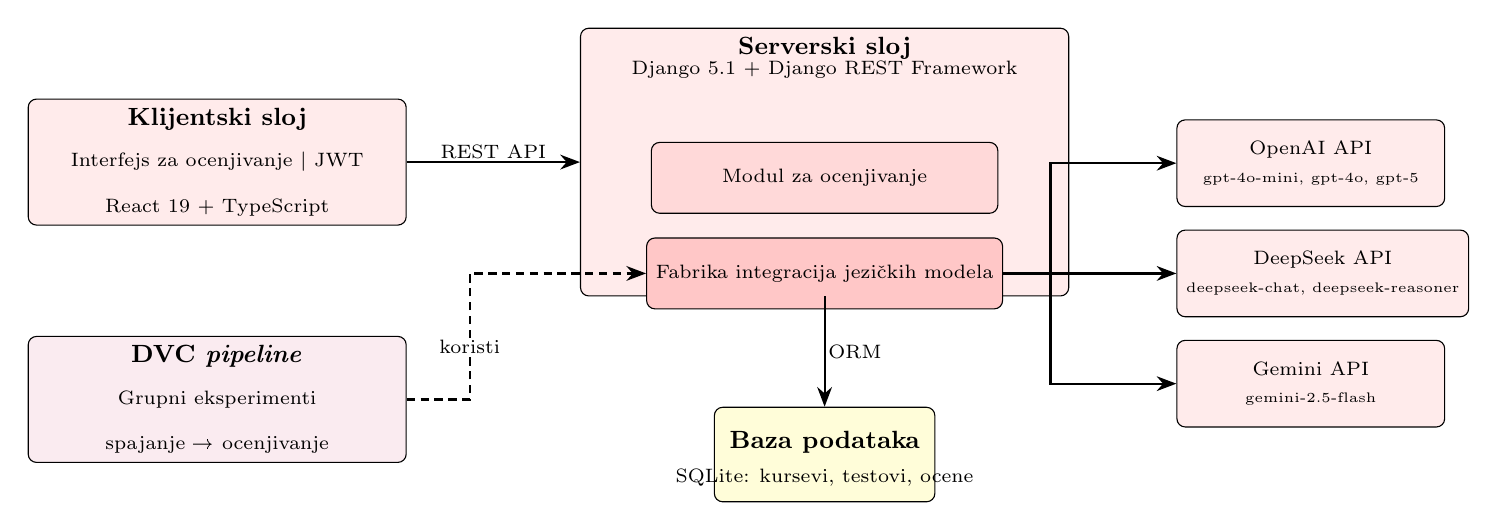
\begin{tikzpicture}[
    node distance=0.6cm and 0.8cm,
    box/.style={draw, rounded corners=3pt, minimum height=0.9cm, text centered, font=\small},
    arr/.style={-{Stealth[length=2.5mm]}, thick},
    darr/.style={-{Stealth[length=2.5mm]}, thick, densely dashed},
    lbl/.style={font=\scriptsize, midway, fill=white, inner sep=1pt},
]

% ---- Klijentski sloj ----
\node[box, fill=red!8, minimum width=4.8cm, minimum height=1.6cm] (fe) {};
\node[font=\small\bfseries, anchor=north] at (fe.north) {Klijentski sloj};
\node[font=\scriptsize, anchor=south] at (fe.south) {React 19 + TypeScript};
\node[font=\scriptsize] at (fe.center) {Interfejs za ocenjivanje \textbar{} JWT};

% ---- Serverski sloj ----
\node[box, fill=red!8, minimum width=6.2cm, minimum height=3.4cm, right=2.2cm of fe] (be) {};
\node[font=\small\bfseries, anchor=north] at (be.north) {Serverski sloj};
\node[font=\scriptsize, anchor=north, yshift=-3mm] at (be.north) {Django 5.1 + Django REST Framework};

% Unutrašnje komponente
\node[box, fill=red!15, minimum width=4.4cm, font=\scriptsize] at ([yshift=-2mm]be.center) (gm) {Modul za ocenjivanje};
\node[box, fill=red!22, minimum width=4.4cm, font=\scriptsize, below=0.3cm of gm] (factory) {Fabrika integracija jezičkih modela};

% ---- Baza podataka ----
\node[box, fill=yellow!15, minimum width=2.8cm, minimum height=1.2cm, below=1.4cm of be] (db) {};
\node[font=\small\bfseries] at ([yshift=1.5mm]db.center) {Baza podataka};
\node[font=\scriptsize] at ([yshift=-3mm]db.center) {SQLite: kursevi, testovi, ocene};

% ---- LLM API-ji ----
\node[box, fill=red!8, minimum width=3.4cm, minimum height=1.1cm, align=center, right=2.2cm of factory, yshift=1.4cm]
  (openai) {\scriptsize OpenAI API\\[-1pt]\tiny gpt-4o-mini, gpt-4o, gpt-5};

\node[box, fill=red!8, minimum width=3.4cm, minimum height=1.1cm, align=center, right=2.2cm of factory]
  (deepseek) {\scriptsize DeepSeek API\\[-1pt]\tiny deepseek-chat, deepseek-reasoner};

\node[box, fill=red!8, minimum width=3.4cm, minimum height=1.1cm, align=center, right=2.2cm of factory, yshift=-1.4cm]
  (gemini) {\scriptsize Gemini API\\[-1pt]\tiny gemini-2.5-flash};

% ---- DVC pipeline ----
\node[box, fill=purple!8, minimum width=4.8cm, minimum height=1.6cm, below=1.4cm of fe] (pipe) {};
\node[font=\small\bfseries, anchor=north] at (pipe.north) {DVC \emph{pipeline}};
\node[font=\scriptsize] at (pipe.center) {Grupni eksperimenti};
\node[font=\scriptsize, anchor=south] at (pipe.south) {spajanje \textrightarrow{} ocenjivanje};

% ---- Strelice ----
\draw[arr] (fe.east) -- node[lbl, above] {REST API} (be.west |- fe.east);
\draw[arr] (be.south) -- node[lbl, right] {ORM} (db.north);
\draw[arr] (factory.east) -- ++(0.6,0) |- (openai.west);
\draw[arr] (factory.east) -- ++(0.6,0) |- (deepseek.west);
\draw[arr] (factory.east) -- ++(0.6,0) |- (gemini.west);
\draw[darr] (pipe.east) -- ++(0.8,0) |- node[lbl, below, pos=0.25] {koristi} (factory.west);

\end{tikzpicture}%
}
\caption{Arhitektura sistema EduGrader.
Klijentski sloj komunicira sa serverskim slojem preko REST API-ja.
Serverski sloj pristupa jezičkim modelima kroz jedinstven integracioni sloj (projektni obrazac fabrika) koji apstrahuje API-je pojedinačnih provajdera.
Sistem za automatizovanu evaluaciju (poglavlje~\ref{sec:pipeline}) koristi isti integracioni sloj za grupne eksperimente.
Integracija Gemini nije korišćena u eksperimentima opisanim u ovom radu.}
\label{fig:architecture}
\end{figure}

\section{Klijentska aplikacija}
\label{sec:webapp}

Klijentska aplikacija je jednostranična aplikacija koja koristi biblioteku React (verzija 19) i jezik TypeScript,
uz Vite kao alat za izgradnju i razvojno okruženje.
Rutiranje je rešeno bibliotekom React Router, kroz koju je aplikacija podeljena na dva modula sa odvojenim pravima pristupa:

\begin{itemize}
    \item \textbf{Nastavnički modul} omogućava pregled predmeta, kreiranje testova i pitanja i pregled rešenih studentskih testova,
    sa prikazom nastavničke ocene uz predlog ocene jezičkog modela za svaki odgovor.
    \item \textbf{Studentski modul} omogućava pregled nadolazećih testova, izradu testa i uvid u rezultate već urađenih testova.
\end{itemize}

Slike~\ref{fig:ui-kurs}--\ref{fig:ui-student} prikazuju tipičan tok rada.
Nastavnik na stranici kursa unosi pitanja sa referentnim odgovorima i od njih sastavlja testove (slika~\ref{fig:ui-kurs}).
Kada student preda test (slika~\ref{fig:ui-student}),
nastavnik pri pregledu za svaki odgovor vidi predlog ocene jezičkog modela i, po potrebi, njegovo obrazloženje,
a konačnu ocenu unosi sam (slika~\ref{fig:ui-ocena}).
Predlog modela je tako samo polazna tačka: nastavnik ga može prihvatiti ili prepraviti, što je princip iz uvoda da je čovek sastavni deo sistema.

Elementi interfejsa su na engleskom, dok su pitanja, referentni odgovori i studentski odgovori na srpskom,
isto kao u eksperimentima iz poglavlja~\ref{sec:rezultati}.

\begin{figure}[htbp]
\centering
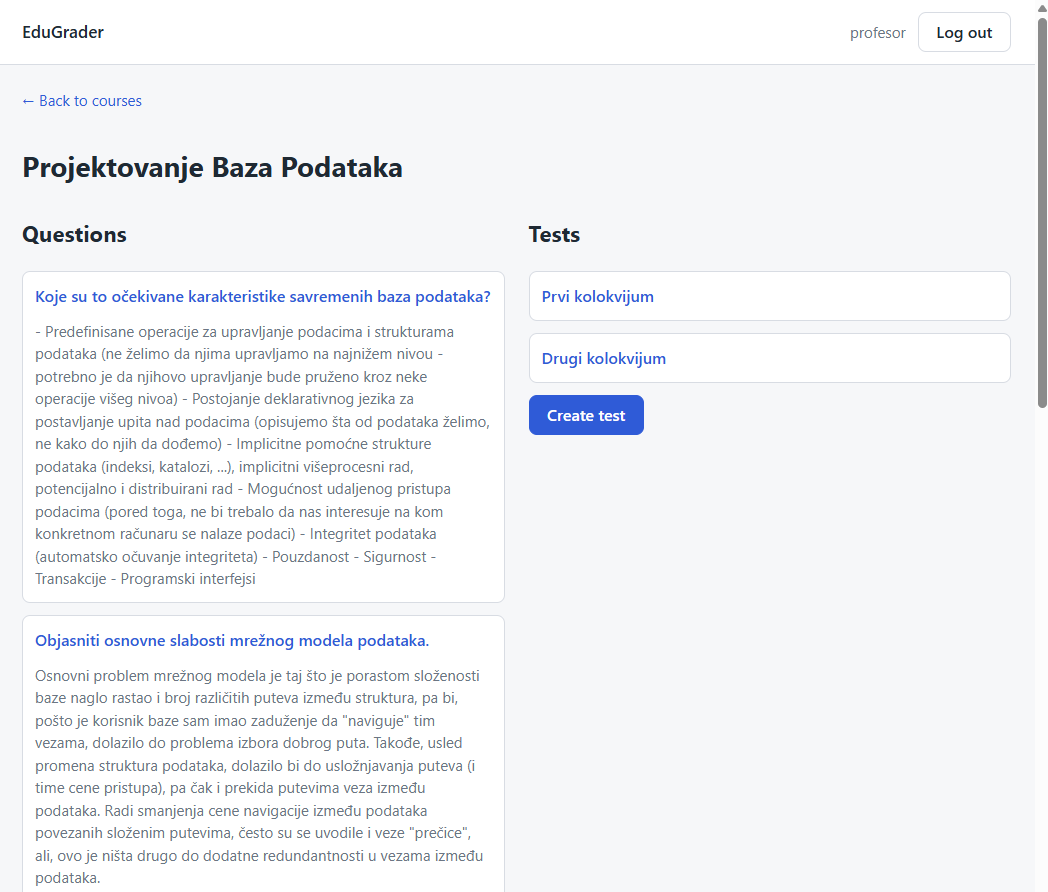
\includegraphics[width=0.8\textwidth]{screenshots/profesor_course.png}
\caption{Nastavnički modul: stranica kursa sa pitanjima, njihovim referentnim odgovorima i listom testova.}
\label{fig:ui-kurs}
\end{figure}

\begin{figure}[htbp]
\centering
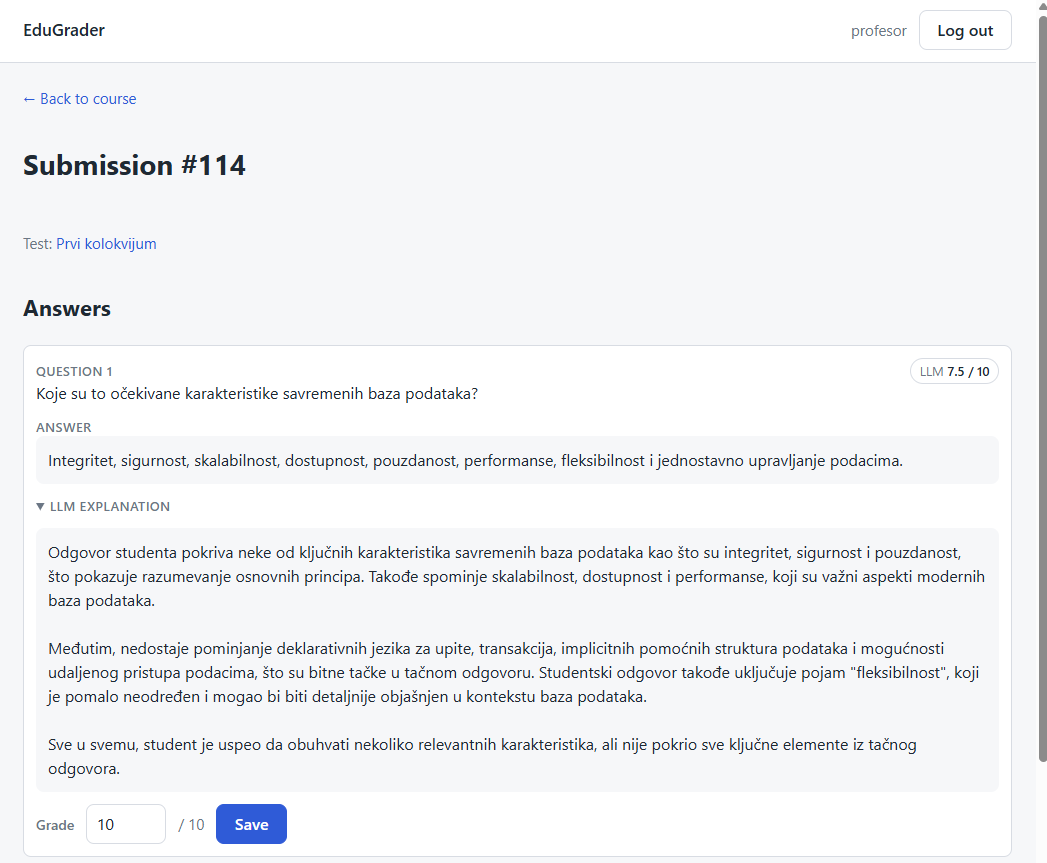
\includegraphics[width=0.8\textwidth]{screenshots/professor_test_submittion_with_llm.png}
\caption{Nastavnički modul: pregled rešenog testa.
Uz svaki odgovor prikazan je predlog ocene jezičkog modela (ovde 7,5 od 10) sa rasklopljenim obrazloženjem,
a konačnu ocenu unosi nastavnik u polje \emph{Grade}.
Na snimku je nastavnik, uprkos predlogu modela od 7,5, uneo konačnu ocenu 10,
što ilustruje da konačna odluka ostaje na njemu.}
\label{fig:ui-ocena}
\end{figure}

\begin{figure}[htbp]
\centering
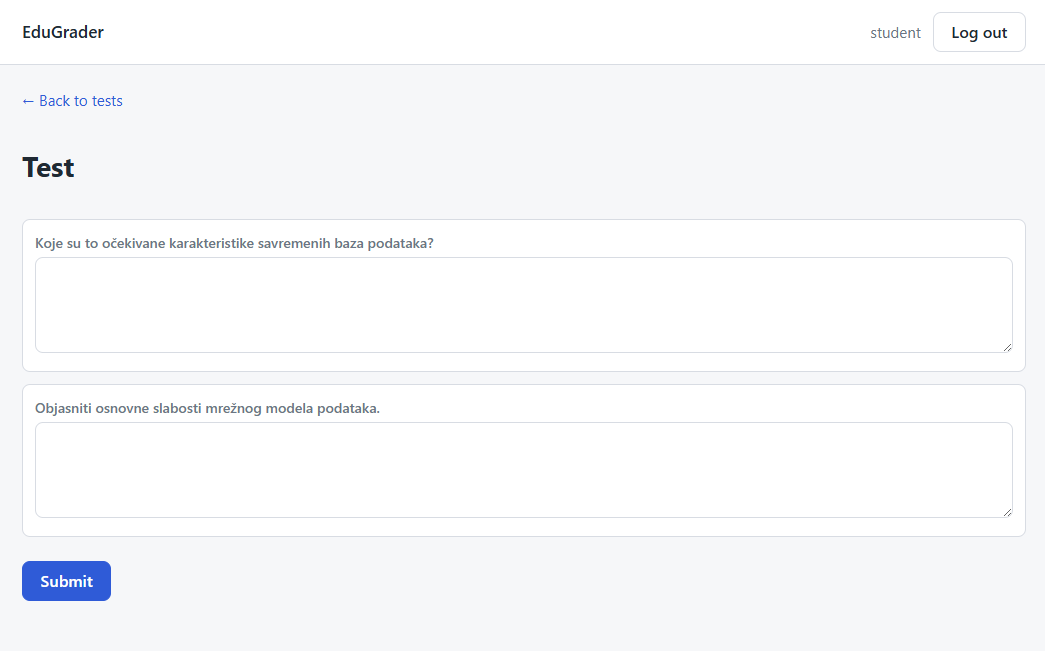
\includegraphics[width=0.8\textwidth]{screenshots/student_test.png}
\caption{Studentski modul: izrada testa.}
\label{fig:ui-student}
\end{figure}

Grupno ocenjivanje se u trenutnoj implementaciji ne pokreće iz korisničkog interfejsa:
logika ocenjivanja izložena je kao funkcije serverskog modula za ocenjivanje,
a eksperimenti opisani u poglavlju~\ref{sec:pipeline} pokreću je kroz \emph{pipeline} u sistemu DVC,
nad podacima pripremljenim u vidu CSV (engl. \emph{comma-separated values}) datoteka.
Izbor modela, režima ocenjivanja i konfiguracije strogosti zadaje se kroz parametarske datoteke tog \emph{pipeline}-a, a ne kroz veb interfejs.

Autentifikacija koristi JWT, koji se čuva u skladištu sesije (engl. \emph{session storage}) pregledača, koje traje dok je kartica otvorena.
Uloge (nastavnik ili student) ugrađene su u njega i na osnovu njih se sprovodi kontrola pristupa rutama.
U razvojnom okruženju Vite server prosleđuje API pozive ka serverskom delu,
dok se u produkciji statička verzija aplikacije poslužuje kroz Nginx.

\section{Serverska aplikacija}

Serverski deo je Django projekat podeljen na tri aplikacije, u skladu sa Django konvencijom razdvajanja odgovornosti:

\begin{itemize}
    \item \textbf{Aplikacija za autentifikaciju} implementira prilagođeni korisnički model sa ulogama student i nastavnik,
    izdavanje i osvežavanje JWT-a,
    kao i klase dozvola (engl. \emph{permission classes}) kojima se pojedinačni API pozivi ograničavaju na odgovarajuću ulogu.
    \item \textbf{Glavna aplikacija} definiše domenske modele, kurs, pitanje,
    test, studentski test i studentski odgovor,
    zajedno sa serijalizatorima i CRUD \emph{endpoint}-ima, adresama REST API-ja preko kojih se izvode pojedinačne operacije nad njima.
    Studentski odgovor čuva i ocenu koju je dodelio nastavnik, što omogućava kasnije poređenje sa ocenama modela.
    \item \textbf{Aplikacija za ocenjivanje} sadrži logiku ocenjivanja i integracije sa jezičkim modelima.
    Za svaki ocenjeni odgovor kreira zapis sa korišćenim promptom, instrukcijama,
    kompletnim odgovorom modela i izdvojenom numeričkom ocenom, pa je svaka ocena naknadno proverljiva.
\end{itemize}

Sistem je zapakovan u Docker kontejnere: jedan kontejner izvršava Django aplikaciju,
a drugi Nginx koji poslužuje klijentsku aplikaciju i prosleđuje API saobraćaj.

\section{Integracija jezičkih modela}
\label{sec:integracije}

Jezičkim modelima pristupa se isključivo preko API-ja provajdera u oblaku;
nijedan model se ne izvršava lokalno.
Više provajdera pokriveno je projektnim obrascem fabrika (engl. \emph{factory}),
sa apstraktnim interfejsom \texttt{LLMIntegration} i metodom \texttt{prompt()} čiji su parametri ulazni tekst,
identifikator modela, sistemske instrukcije i temperatura.
Metoda vraća par: izdvojeni tekstualni odgovor i kompletan odgovor API-ja, koji se čuva radi sledivosti.

Implementirane su tri integracije, kao tri implementacije zajedničkog interfejsa
(\texttt{LLMIntegration}), dostupne istovremeno i birane po simboličkom imenu:

\begin{itemize}
    \item \textbf{OpenAI}, koristi zvanični OpenAI Python SDK (engl. \emph{software development kit}).
    Podržani modeli: \texttt{gpt-\allowbreak 4o-\allowbreak mini}, \texttt{gpt-4o} i \texttt{gpt-5}.
    \item \textbf{DeepSeek}, koristi OpenAI-kompatibilni API \emph{endpoint} preko istog SDK-a, sa promenjenom baznom adresom.
    Podržani modeli: \texttt{deepseek-chat} (V3) i \texttt{deepseek-reasoner} (R1).
    \item \textbf{Google Gemini}, koristi zvanični Google GenAI Python SDK.
    Podrazumevani model: \texttt{gemini-2.5-flash}.
    U aplikaciji služi za generisanje simuliranih studentskih odgovora pri testiranju
    i nije korišćena u eksperimentima opisanim u ovom radu.
\end{itemize}

Fabrička funkcija instancira odgovarajuću klasu na osnovu simboličkog imena integracije
(\texttt{openai}, \texttt{deepseek}, \texttt{gemini}).
Nov provajder se tako dodaje implementacijom jedne klase, bez izmena u logici ocenjivanja;
isti mehanizam koriste i veb aplikacija i sistem za automatizovanu evaluaciju iz poglavlja~\ref{sec:pipeline}.
API ključevi čuvaju se kao promenljive okruženja i nikada nisu ugrađeni u izvorni kod.

% 4. Sistem za automatizovanu evaluaciju modela
\section{Sistem za automatizovanu evaluaciju modela}
\label{sec:pipeline}

Za potrebe evaluacije opisane u poglavlju~\ref{sec:metodologija} razvijen je zaseban sistem za automatizovanu evaluaciju modela, organizovan kao DVC \emph{pipeline} (engl. \emph{Data Version Control})\footnote{\url{https://dvc.org}}.
DVC omogućava deklarativno opisivanje faza obrade sa eksplicitnim zavisnostima i izlazima: svaka faza se ponovo izvršava samo ako su se njeni ulazi ili parametri promenili, što eksperimente čini reproducibilnim i štedi troškove API poziva.

\subsection{Format ulaznih podataka}

Svaki od devet skupova podataka (pet kurseva, pri čemu su za pojedine kurseve obuhvaćeni odvojeni ispitni rokovi) opisan je dvema CSV datotekama:

\begin{itemize}
    \item \texttt{questions.csv}, po jedan red za svako pitanje, sa kolonama: identifikator pitanja, tekst pitanja, tačan odgovor nastavnika i adresa nastavnog materijala (PDF udžbenika) iz koga je pitanje postavljeno;
    \item \texttt{student\_answers.csv}, po jedan red za svaki studentski odgovor, sa kolonama: identifikator studenta, identifikator pitanja, ocena nastavnika (0--10) i tekst odgovora.
\end{itemize}

\subsection{Faze obrade}

Prva faza (\emph{spajanje ulaza}) validira i spaja ove dve datoteke u jedinstvenu tabelu.
Validacija obuhvata proveru obaveznih kolona, jedinstvenosti identifikatora pitanja, nepraznosti svih polja i kompletnosti podataka, svaki student mora imati odgovor na svako pitanje; u suprotnom se obrada prekida sa opisom greške.
Ovakve stroge provere pokazale su se ključnim za kvalitet eksperimenata, jer su greške u ručno pripremanim podacima otkrivane pre nego što bi izazvale skupe, delimično neispravne eksperimente.

Druga faza (\emph{ocenjivanje}) za svaki red spojene tabele konstruiše prompt i poziva izabrani jezički model preko integracionog sloja iz odeljka~\ref{sec:integracije}.
Postoje tri varijante ove faze, od kojih dve odgovaraju režimima ocenjivanja iz odeljka~\ref{sec:modeli}:

\begin{itemize}
    \item \textbf{PRA varijanta} u prompt uključuje pitanje, tačan odgovor nastavnika i studentski odgovor.
    \item \textbf{GRA varijanta} umesto tačnog odgovora nastavnika koristi referentni odgovor koji model sam generiše iz nastavnog materijala.
    Ovo je dvostepen postupak: u prvom koraku materijal se preuzima sa zadate adrese kao PDF, tekst se izdvaja bibliotekom PyPDF2 i kešira na disku (po heš vrednosti adrese, tako da se svaki udžbenik preuzima i obrađuje samo jednom), a model iz njega konstruiše koncizan referentni odgovor dužine dve do pet rečenica.
    U drugom koraku studentski odgovor ocenjuje se u odnosu na taj generisani standard, istim postupkom kao u PRA varijanti.
    Time se za svaki skup podataka dobija tabela pitanja u kojoj su nastavnički referentni odgovori zamenjeni generisanim, pa se ocenjivanje sprovodi ponovnom upotrebom iste komponente kao u PRA varijanti.
    \item \textbf{Varijanta sa nastavnim materijalom u promptu} ne koristi referentni odgovor, već ceo izvučeni tekst udžbenika umeće u svaki prompt za ocenjivanje.
    Ova varijanta razmatrana je, ali nije sprovedena do kraja i njeni rezultati se ne koriste u analizi; razlozi su izloženi u odeljku~\ref{sec:rezim-udzbenik}.
\end{itemize}

U svim varijantama sistemska instrukcija se sastoji od prompta strogosti (blag, neutralan ili strog; dodatak~\ref{app:promptovi}) i fiksnog uputstva o formatu izlaza: prvi red odgovora mora sadržati samo ocenu na skali 0--100, a ostatak obrazloženje.
Temperatura se ne postavlja eksplicitno, pa modeli rade na podrazumevanoj vrednosti svog provajdera.
Numerička ocena se parsira iz prvog reda odgovora; skala 0--100 naknadno se preslikava na skalu 0--10 radi poređenja sa ocenama nastavnika.
Ako parsiranje ne uspe, poziv se ponavlja, do tri pokušaja ukupno; ako API poziv privremeno otkaže, ponavljanju prethodi rastuće odlaganje.
Trajno neuspešni redovi označavaju se specijalnom negativnom vrednošću i isključuju iz analize.

\subsection{Automatizacija eksperimenata i analiza}

Potpuni eksperiment obuhvata petnaest kombinacija (pet modela $\times$ tri nivoa strogosti) nad svih devet skupova podataka, dakle 135 pokretanja po režimu ocenjivanja.
Pomoćna skripta automatizuje ovaj proces: za svaku kombinaciju upisuje izbor modela i strogosti u parametarsku datoteku i ponovo pokreće DVC \emph{pipeline}, pri čemu ime svake izlazne datoteke kodira konfiguraciju (strogost, model i režim) kojom je proizvedena.
Svaka kombinacija pokrenuta je jednom, pa rezultati ne obuhvataju procenu varijabilnosti između ponovljenih pokretanja istog modela.

Završna analitička skripta prolazi kroz sve ocenjene datoteke, uparuje ocene modela sa ocenama nastavnika i računa metrike opisane u odeljku~\ref{sec:metrike}, Pirsonov koeficijent korelacije, odnos prosečnih ocena, RMSE i odnos RMSE/STDDEV, po svakoj kombinaciji skupa podataka, modela, strogosti i režima.
Rezultati se objedinjuju u zbirnu tabelu iz koje su izvedeni rezultati prikazani u poglavlju~\ref{sec:rezultati}.

% 4. Metodologija evaluacije
\section{Metodologija evaluacije}
\label{sec:metodologija}

EduGrader je projektovan kao platforma za ocenjivanje uz podršku veštačke inteligencije koja velike jezičke modele uključuje u tok provere znanja pod nadzorom nastavnika.
Primarni cilj sistema je unapređenje efikasnosti i doslednosti ocenjivanja uz očuvanje pedagoške transparentnosti i ljudske odgovornosti.
U ovom poglavlju opisana je metodologija evaluacije pouzdanosti ocena koje EduGrader generiše, skupovi podataka na kojima je sistem testiran i konfiguracije modela obuhvaćene eksperimentima.

\subsection{Metrike i evaluacija}
\label{sec:metrike}

Da bi se procenilo slaganje ocena generisanih veštačkom inteligencijom sa ljudskim sudom, izlazi sistema EduGrader upoređeni su sa ocenama koje su dodelila dva univerzitetska nastavnika.
Svaki nastavnik je ocenio drugačiji podskup od ukupno 583 odgovora, pri čemu su podskupovi određeni kursevima na kojima nastavnici predaju.
Ovakva postavka omogućila je poređenje performansi sistema sa više ljudskih ocenjivača, umesto sa jednim jedinstvenim standardom.
Svaki odgovor ocenjen je prema standardnim kriterijumima ocenjivanja koji se koriste na datom kursu.
Ocene su dodeljivane na skali 0--10, na osnovu stepena konceptualne tačnosti i potpunosti odgovora.
Nastavnici su uzimali u obzir da li je student ispravno identifikovao ključne koncepte, da li nedostaju važni elementi i da li je rezonovanje delimično tačno, ali nepotpuno.
Odgovori koji demonstriraju ispravne osnovne ideje dobijali su delimične poene čak i kada nedostaju terminologija, struktura ili pojedini detalji, dok su suštinski netačni odgovori dobijali niske ocene ili nula poena.
Za svaki odgovor, ocena koju je dodelio nastavnik zadužen za kurs tretirana je kao referentna ocena i upoređena sa ocenom sistema, preslikanom na istu skalu 0--10, pomoću metrika opisanih u nastavku.

Korišćena su tri statistička pokazatelja koji obuhvataju komplementarne aspekte pouzdanosti ocenjivanja: Pirsonov koeficijent korelacije (PCC), odnos prosečnih ocena (engl. \emph{Mean Ratio}) i odnos korena srednje kvadratne greške i standardne devijacije (RMSE/STDDEV).

PCC~\cite{sedgwick2012pearson} meri jačinu linearne povezanosti između ocena koje su dodelili ljudi i ocena koje je dodelio sistem.
Koeficijent uzima vrednosti od $-1$ do $+1$, gde $+1$ označava savršenu pozitivnu linearnu vezu, $0$ odsustvo linearne veze, a $-1$ savršenu negativnu linearnu vezu.
Važno je istaći da PCC meri linearnu povezanost, a ne apsolutno slaganje: sistem koji sve ocene dosledno umanjuje za istu vrednost postigao bi savršenu korelaciju uz očigledno pogrešne ocene.
Iz tog razloga, PCC je dopunjen metrikama koje obuhvataju apsolutna odstupanja između ocena sistema i nastavnika.

Odnos prosečnih ocena sažima opšte tendencije u ocenjivanju.
Razlike između prosečne ocene sistema i prosečne ocene nastavnika ukazuju na sistematsku blagost ili strogost, ali ne odražavaju usklađenost u variranju ocena.

Koren srednje kvadratne greške (RMSE)~\cite{hodson2022root} obuhvata prosečnu veličinu razlika između ljudskih ocena i ocena sistema; manja vrednost RMSE ukazuje na jače slaganje.
Odnos RMSE/STDDEV~\cite{chai2014root} meri koliko se ocene sistema slažu sa ljudskim ocenama u odnosu na prirodnu varijabilnost samih ljudskih ocena, odnosno, da li su odstupanja sistema od ljudskog suda mala u poređenju sa tim koliko ljudske ocene uopšte variraju.
Vrednost odnosa RMSE/STDDEV blizu $0$ ukazuje na veoma visoko slaganje, vrednost oko $1$ znači da su odstupanja sistema uporediva sa tipičnom varijabilnošću ljudskog ocenjivanja, dok vrednost veća od $1$ sugeriše da se ocene sistema razlikuju od ljudskih više nego što se ljudi razlikuju međusobno.

\subsection{Prikupljanje podataka}
\label{sec:podaci}

Empirijska evaluacija sistema EduGrader sprovedena je na autentičnim odgovorima sa teorijskih ispita, prikupljenim tokom više ispitnih rokova na dva univerziteta u Srbiji.

Dobijeni skup podataka obuhvata \textbf{pet univerzitetskih kurseva} i pokriva više akademskih nivoa, uključujući osnovne i master studije.
Sadrži mešavinu konceptualnih pitanja i zadataka vezanih za programiranje, čime pruža raznovrstan i heterogen reper za evaluaciju sistema za automatsko ocenjivanje.
Kursevi obuhvaćeni skupom podataka su:

\begin{itemize}
    \item Programiranje 2 (Prog 2): kurs prve godine osnovnih studija, Matematički fakultet, Univerzitet u Beogradu;
    \item Tehničko i naučno pisanje (TSW): kurs prve godine osnovnih studija, Matematički fakultet, Univerzitet u Beogradu;
    \item Veb programiranje (WP): kurs četvrte godine osnovnih studija, Matematički fakultet, Univerzitet u Beogradu;
    \item Digitalno čuvanje podataka (DDS): kurs master studija, Univerzitet umetnosti;
    \item HTML5 i JavaScript za video-igre (HTML5): kurs master studija, Univerzitet umetnosti.
\end{itemize}

Podaci su organizovani po ispitnim rokovima, a ne po kursevima: ukupno devet skupova podataka odgovara devet ispitnih rokova, koji se grupišu u pet navedenih kurseva (tri roka za Programiranje 2, po dva za Tehničko i naučno pisanje i Veb programiranje, i po jedan za Digitalno čuvanje podataka i HTML5).
Svi eksperimenti izvršavaju se nad pojedinačnim rokovima, dok se rezultati u poglavlju~\ref{sec:rezultati} prikazuju objedinjeno i po kursevima.

Uz svaki kurs, skup podataka sadrži studentske odgovore, ocene koje su dodelili nastavnici, referentne odgovore (kada su dostupni), napomene nastavnika i relevantne nastavne materijale korišćene u pripremi ispita.
Ukupno, skup sadrži \textbf{583 studentska odgovora}, što predstavlja realističan reper za evaluaciju doslednosti ocenjivanja kroz različite discipline, akademske nivoe i formate pitanja.
U zavisnosti od kursa, odgovori uključuju \textbf{kratka tekstualna objašnjenja} i \textbf{odgovore u obliku koda}.
Tabela~\ref{tab:dataset} sumira strukturu skupa podataka, uključujući broj odgovora i njihove tipove za svaki kurs.

Radi bolje karakterizacije podataka, dodatno je prikazana raspodela tipova odgovora i prosečna dužina odgovora.
Ove statistike daju uvid u varijabilnost složenosti odgovora i pomažu u kontekstualizaciji težine automatskog ocenjivanja kroz različite formate pitanja.
Pored raspodele tipova odgovora, analizirana je i tipična dužina odgovora, kako referentnih rešenja koja su pripremili nastavnici, tako i automatski generisanih referentnih odgovora i samih studentskih odgovora.
Ova informacija je relevantna jer dužina odgovora može uticati na težinu automatskog ocenjivanja.

Tabela~\ref{tab:response_length} takođe pokazuje da su generisani referentni odgovori često znatno duži od odgovora koje su pripremili nastavnici, naročito kod pitanja gde se očekuju kratki odgovori.
Na više kurseva nastavnici očekuju sažete odgovore (npr.\ jedan izraz ili kratku konstataciju), dok odgovori koje generišu jezički modeli po pravilu uključuju i dodatna objašnjenja zašto je odgovor tačan.
Kao rezultat, generisani odgovori sadrže više kontekstualnih informacija nego što izvorno ispitno pitanje strogo zahteva.

\begin{table}[ht]
\centering
\caption{Struktura skupa podataka po kursevima (broj studentskih odgovora po tipu pitanja)}
\label{tab:dataset}
\resizebox{\columnwidth}{!}{%
\begin{tabular}{lccc}
\toprule
\textbf{Kurs} &
\textbf{Odgovori} &
\textbf{Kratak tekst} &
\textbf{Kod} \\
\midrule
Programiranje 2 (Prog 2) & 477 & 362 & 115 \\
Tehničko i naučno pisanje (TSW) & 40 & 20 & 20 \\
Veb programiranje (WP) & 46 & 40 & 6 \\
Digitalno čuvanje podataka (DDS) & 10 & 10 & 0 \\
HTML5 i JavaScript za video-igre (HTML5) & 10 & 10 & 0 \\
\midrule
\textbf{Ukupno} & \textbf{583} & \textbf{442 (75{,}8\%)} & \textbf{141 (24{,}2\%)} \\
\bottomrule
\end{tabular}
}
\end{table}

Pitanje je svrstano u kategoriju \emph{kod} ukoliko se od studenta traži da napiše programski kod, izraz ili \LaTeX{} naredbu, a u kategoriju \emph{kratak tekst} ukoliko se očekuje prozni odgovor, čak i kada se u samom pitanju navodi isečak koda.

\begin{table}[ht]
\centering
\caption{Prosečna dužina odgovora po tipu pitanja i izvoru odgovora}
\label{tab:response_length}
\resizebox{\columnwidth}{!}{%
\begin{tabular}{lcccccc}
\toprule
\textbf{Tip pitanja} &
\textbf{\shortstack{Odgovor nastavnika\\pros.\ reči}} &
\textbf{\shortstack{Odgovor nastavnika\\pros.\ znakova}} &
\textbf{\shortstack{Generisani odgovor\\pros.\ reči}} &
\textbf{\shortstack{Generisani odgovor\\pros.\ znakova}} &
\textbf{\shortstack{Studentski odgovor\\pros.\ reči}} &
\textbf{\shortstack{Studentski odgovor\\pros.\ znakova}} \\
\midrule
Kratak tekst & 20.9 & 130.5 & 201.7 & 1341.9 & 24.7 & 143.2 \\
Kod          & 22.2 & 137.4 & 162.7 & 1144.3 & 15.9 & 102.5 \\
\bottomrule
\end{tabular}
}
\end{table}

\subsection{Modeli i konfiguracije}
\label{sec:modeli}

EduGrader koristi višemodelski pristup ocenjivanju koji uključuje i modele opšte namene i modele optimizovane za rezonovanje:
\begin{itemize}
    \item standardni modeli: GPT-4o, GPT-4o-mini, DeepSeek-Chat;
    \item modeli za rezonovanje: GPT-5, DeepSeek-Reasoner.
\end{itemize}
Svaki model evaluiran je u tri konfiguracije strogosti ocenjivanja: blagoj, neutralnoj i strogoj.
Ove konfiguracije realizovane su pažljivo projektovanim promptovima koji simuliraju različite filozofije ocenjivanja uobičajene u akademskoj praksi.
Na primer, stroga konfiguracija predstavlja model kao „strogog profesora visokoakademske institucije'', usmerava mu pažnju na stavke koje se ne poklapaju sa studentskim odgovorom i zadaje eksplicitnu meru kazne (oduzimanje petine poena po nepoklapanju), dok blaga konfiguracija usmerava pažnju na stavke koje se poklapaju.
Neutralna konfiguracija ne uvodi nikakvo dodatno pravilo i predstavlja osnovnu postavku ocenjivanja.
Puni tekstovi svih promptova navedeni su u dodatku~\ref{app:promptovi}.
Ovakav dizajn odražava nalaze prethodnih studija koje pokazuju da i ljudski ocenjivači značajno variraju u strogosti~\cite{jukiewicz2024future}.

Pored toga, EduGrader podržava dva komplementarna režima ocenjivanja:
\begin{itemize}
    \item PRA, u kome se studentski odgovori porede sa tačnim odgovorima i napomenama za ocenjivanje koje je pripremio nastavnik;
    \item GRA, u kome model najpre generiše referentni odgovor na osnovu priloženih nastavnih materijala, a zatim studentski odgovor ocenjuje u odnosu na taj generisani standard.
\end{itemize}
Ovakav dvorežimski dizajn omogućava evaluaciju kako u scenarijima sa dobro definisanim ključem za ocenjivanje, tako i u situacijama kada nastavnici ne obezbeđuju eksplicitna referentna rešenja.

Svi eksperimenti sprovedeni su na srpskom jeziku, uključujući ispitna pitanja, studentske odgovore i referentne odgovore.
Budući da je srpski jezik sa ograničenim resursima, slabo zastupljen u podacima na kojima se veliki jezički modeli obučavaju, ovo istraživanje proširuje oblast ocenjivanja uz podršku veštačke inteligencije izvan dominantnog engleskog konteksta.

\subsection{Razmatran treći režim: ocenjivanje direktno iz nastavnog materijala}
\label{sec:rezim-udzbenik}

Pored dva režima opisana u prethodnom odeljku, razmatran je i treći pristup, u kome se referentni odgovor uopšte ne koristi.
U njemu se ceo tekst nastavnog materijala, izdvojen iz PDF udžbenika, umeće direktno u prompt zajedno sa pitanjem i studentskim odgovorom, a od modela se traži da odgovor oceni oslanjajući se isključivo na taj materijal.
Za razliku od GRA režima, gde se udžbenik koristi jednom, da bi se iz njega izveo kratak referentni odgovor, ovde udžbenik ulazi u svaki pojedinačni poziv za ocenjivanje.
Pristup je motivisan idejom da bi izostavljanje posredničkog koraka moglo da spreči gubitak informacija pri generisanju referentnog odgovora, naročito kod pitanja čiji odgovor zahteva širi kontekst.

Ovaj režim implementiran je i pokrenut, ali \textbf{nije sproveden do kraja}, i njegovi rezultati se u ovom radu ne koriste za izvođenje zaključaka.
Razlog je cena: budući da ceo udžbenik ulazi u svaki poziv, veličina prompta raste za red veličine.
Medijana broja tokena u promptu iznosila je oko $14\,500$ za kurs Programiranje 2, naspram oko $260$ tokena u PRA režimu za istu grupu pitanja, dakle približno \textbf{55 puta više}.
Sprovedeni deo eksperimenta potrošio je oko $38{,}5$ miliona tokena u promptovima, pri čemu je pokrio samo oko trećine planirane mreže konfiguracija; njeno kompletiranje zahtevalo bi približno $119$ miliona tokena.

Zbog toga su u ovom režimu evaluirani samo modeli GPT-4o-mini i GPT-4o, dok modeli usmereni na rezonovanje (GPT-5 i DeepSeek-Reasoner) i model DeepSeek-Chat nisu pokretani.
Ocenjivanje je u potpunosti sprovedeno jedino za model GPT-4o-mini, kroz sve tri konfiguracije strogosti; za model GPT-4o blaga konfiguracija ostala je praktično nepokrenuta, a stroga nepotpuna.
Ocenjene datoteke zadržane su u repozitorijumu radi sledivosti, ali se, u skladu sa nepotpunom pokrivenošću, u poglavlju~\ref{sec:rezultati} ne prikazuju uz rezultate PRA i GRA režima.
Ograničenja koja iz ovoga slede razmatraju se u odeljku~\ref{sec:ogranicenja}.

% 5. Rezultati
\section{Rezultati}
\label{sec:rezultati}

Tabele~\ref{tab:pra_results} i~\ref{tab:gra_results} sumiraju rezultate za PRA odnosno GRA režim kroz tri pokazatelja: PCC kao meru linearne povezanosti sa ljudskim ocenama, odnos prosečnih ocena (prosečna ocena sistema / prosečna ocena nastavnika) kao pokazatelj sistematskog odstupanja (blagosti ili strogosti) i odnos RMSE/STDDEV kao meru relativnog odstupanja od varijabilnosti ljudskog ocenjivanja.
Sve vrednosti izračunate su nad objedinjenim skupom svih ocenjenih odgovora, a ne kao prosek vrednosti po pojedinačnim skupovima podataka.

Svaka konfiguracija (model $\times$ strogost $\times$ režim) pokrenuta je jednom, pa rezultati odražavaju jedno uzorkovanje iz svakog modela.
Temperatura se u glavnoj mreži konfiguracija ne varira:
modeli porodice GPT rade na podrazumevanoj vrednosti svog provajdera,
a modelima DeepSeek prosleđuje se vrednost $0$ (odeljak~\ref{sec:pipeline}).
Njen uticaj ispitan je odvojeno, na podskupu odgovora, u odeljku~\ref{sec:rezultati-temperatura}.

\subsection{Performanse modela}
\label{sec:performanse}

\begin{table}[ht]
\centering
\caption{Metrike performansi za PRA režim kroz modele i konfiguracije strogosti.
Najbolji rezultati za svaku metriku i konfiguraciju strogosti označeni su podebljano.
Za odnos prosečnih ocena najboljom se smatra vrednost najbliža 1{,}0.}
\label{tab:pra_results}
\resizebox{\textwidth}{!}{%
\begin{tabular}{l ccc ccc ccc}
\toprule
\textbf{Model} &
\multicolumn{3}{c}{\textbf{PCC}} &
\multicolumn{3}{c}{\textbf{Odnos proseka}} &
\multicolumn{3}{c}{\textbf{RMSE/STDDEV}} \\
\cmidrule(lr){2-4}
\cmidrule(lr){5-7}
\cmidrule(lr){8-10}
& blag & neutr. & strog
& blag & neutr. & strog
& blag & neutr. & strog \\
\midrule
GPT-4o-mini       & 0{,}82 & 0{,}80 & 0{,}77 & \textbf{0{,}96} & 0{,}93 & \textbf{0{,}97} & 0{,}57 & 0{,}61 & 0{,}65 \\
GPT-4o            & 0{,}80 & 0{,}84 & 0{,}79 & 0{,}90 & \textbf{1{,}00} & 0{,}79 & 0{,}65 & 0{,}55 & 0{,}74 \\
GPT-5             & \textbf{0{,}89} & \textbf{0{,}88} & 0{,}77 & 0{,}94 & 0{,}91 & \textbf{1{,}00} & \textbf{0{,}47} & \textbf{0{,}50} & 0{,}65 \\
DeepSeek-Chat     & 0{,}81 & 0{,}82 & \textbf{0{,}83} & 0{,}80 & 0{,}84 & 0{,}86 & 0{,}71 & 0{,}65 & \textbf{0{,}61} \\
DeepSeek-Reasoner & 0{,}87 & 0{,}86 & 0{,}78 & 0{,}88 & 0{,}86 & 0{,}95 & 0{,}53 & 0{,}56 & 0{,}63 \\
\bottomrule
\end{tabular}
}
\end{table}

Vrednosti u tabeli~\ref{tab:pra_results} izračunate su nad svih 583 odgovora, osim u dva slučaja u kojima ocenjivanje nije uspelo za sve odgovore: neutralna konfiguracija modela GPT-4o obuhvata 399 odgovora, a neutralna konfiguracija modela DeepSeek-Reasoner 555 odgovora.\footnote{Nedostajuće ocene posledica su prekinutog pokretanja, odnosno trajno neuspešnih API poziva, koji se prema opisu iz odeljka~\ref{sec:pipeline} označavaju i isključuju iz analize.}

Modeli usmereni na rezonovanje pokazuju najjače ukupne performanse.
GPT-5 postiže najvišu korelaciju u blagoj i neutralnoj konfiguraciji (PCC $=0{,}89$ i $0{,}88$) uz najniže odnose RMSE/STDDEV ($0{,}47$ i $0{,}50$), a DeepSeek-Reasoner ga prati u stopu ($0{,}87$ i $0{,}86$).
GPT-4o je konkurentan u neutralnoj konfiguraciji (PCC $=0{,}84$), gde postiže i odnos prosečnih ocena praktično jednak $1{,}0$, dok su GPT-4o-mini i DeepSeek-Chat dosledno nešto slabiji.

Stroga konfiguracija menja poredak: u njoj najvišu korelaciju postiže DeepSeek-Chat (PCC $=0{,}83$), a GPT-5 i GPT-4o-mini padaju na $0{,}77$.
DeepSeek-Chat je pri tom jedini model kod koga korelacija monotono raste sa strogošću ($0{,}81 \rightarrow 0{,}82 \rightarrow 0{,}83$), dok kod svih ostalih stroga konfiguracija daje najniže vrednosti.
Kod modela GPT-4o stroga konfiguracija istovremeno unosi izraženo sistematsko odstupanje naniže (odnos proseka $0{,}79$), što znači da model ocenjuje znatno strože od nastavnika.

Odnosi prosečnih ocena pokazuju da modeli iz porodice GPT ostaju bliži prosecima ljudskog ocenjivanja od modela DeepSeek.
DeepSeek-Chat dosledno ocenjuje konzervativnije od nastavnika u svim konfiguracijama (odnosi $0{,}80$--$0{,}86$), dok GPT-4o-mini ostaje u rasponu $0{,}93$--$0{,}97$.

\begin{table}[ht]
\centering
\caption{Metrike performansi za GRA režim.
Najbolji rezultati za svaku metriku i konfiguraciju strogosti označeni su podebljano.}
\label{tab:gra_results}
\resizebox{\textwidth}{!}{%
\begin{tabular}{l ccc ccc ccc}
\toprule
\textbf{Model} &
\multicolumn{3}{c}{\textbf{PCC}} &
\multicolumn{3}{c}{\textbf{Odnos proseka}} &
\multicolumn{3}{c}{\textbf{RMSE/STDDEV}} \\
\cmidrule(lr){2-4}
\cmidrule(lr){5-7}
\cmidrule(lr){8-10}
& blag & neutr. & strog
& blag & neutr. & strog
& blag & neutr. & strog \\
\midrule
GPT-4o-mini       & 0{,}63 & 0{,}65 & 0{,}61 & 0{,}79 & 0{,}77 & 0{,}82 & 0{,}85 & 0{,}84 & 0{,}84 \\
GPT-4o            & 0{,}69 & 0{,}75 & 0{,}65 & 0{,}78 & \textbf{0{,}88} & 0{,}61 & 0{,}86 & 0{,}69 & 1{,}04 \\
GPT-5             & \textbf{0{,}85} & \textbf{0{,}84} & \textbf{0{,}73} & \textbf{0{,}87} & 0{,}83 & \textbf{0{,}89} & \textbf{0{,}57} & \textbf{0{,}61} & \textbf{0{,}73} \\
DeepSeek-Chat     & 0{,}43 & 0{,}50 & 0{,}47 & 0{,}37 & 0{,}52 & 0{,}42 & 1{,}42 & 1{,}22 & 1{,}34 \\
DeepSeek-Reasoner & 0{,}79 & 0{,}79 & 0{,}70 & 0{,}81 & 0{,}77 & 0{,}87 & 0{,}70 & 0{,}72 & 0{,}77 \\
\bottomrule
\end{tabular}
}
\end{table}

Tabela~\ref{tab:gra_results} prikazuje rezultate za \textbf{GRA} režim, u kome referentne odgovore automatski generiše jezički model umesto nastavnika.
Očekivano, rezultati u GRA režimu su niži od onih dobijenih sa referentnim odgovorima nastavnika.
Ovaj pad performansi odražava dodatnu neizvesnost koju unose automatski generisani referentni odgovori, koji se mogu razlikovati po strukturi, formulaciji ili nivou detalja od rešenja koje je nastavnik imao na umu.

Modeli za rezonovanje najbolje podnose prelazak u GRA režim.
GPT-5 zadržava snažno slaganje (PCC $=0{,}85$ u blagoj i $0{,}84$ u neutralnoj konfiguraciji) i jedini u svim konfiguracijama drži RMSE/STDDEV ispod $0{,}75$, a DeepSeek-Reasoner ostaje na $0{,}79$.
To sugeriše da su sposobniji modeli za rezonovanje istovremeno bolji i u generisanju prikladnih referentnih odgovora i u ocenjivanju u odnosu na njih.

DeepSeek-Chat je u GRA režimu izrazito neupotrebljiv: korelacija pada na $0{,}43$--$0{,}50$, odnos prosečnih ocena na $0{,}37$--$0{,}52$, a RMSE/STDDEV prelazi $1{,}2$ u svim konfiguracijama, dakle njegove ocene odstupaju od ljudskih više nego što ljudske ocene variraju međusobno.
GPT-4o pokazuje isti problem u strogoj konfiguraciji (RMSE/STDDEV $=1{,}04$, odnos proseka $0{,}61$).

\subsection{Poređenje PRA i GRA režima kroz modele i nivoe strogosti}
\label{sec:pra-vs-gra}

Kroz sve evaluirane modele i konfiguracije strogosti, PRA režim dosledno nadmašuje GRA režim, i po korelaciji sa ljudskim ocenama i po normalizovanim odnosima greške.

\subsubsection{Korelacija sa ljudskim ocenjivanjem}

Prelaskom u GRA režim korelacije opadaju kod svih modela, ali neujednačeno.
Kod modela GPT-5 pad je najmanji (sa $0{,}88$ na $0{,}84$ u neutralnoj konfiguraciji), a kod modela DeepSeek-Chat najveći (sa $0{,}82$ na $0{,}50$).
Ova razlika pokazuje da kvalitet automatski generisanog referentnog odgovora, a ne samo sposobnost ocenjivanja, presudno određuje performanse u GRA režimu.

\subsubsection{Uticaj konfiguracije strogosti}

Ne postoji konfiguracija strogosti koja je najbolja za sve modele, i optimalna konfiguracija se razlikuje između dva režima.
U PRA režimu najvišu korelaciju blaga konfiguracija daje kod modela GPT-5, GPT-4o-mini i DeepSeek-Reasoner, neutralna kod modela GPT-4o, a stroga kod modela DeepSeek-Chat.
U GRA režimu neutralna konfiguracija je najbolja kod svih modela osim GPT-5, kod koga je najbolja blaga; kod modela DeepSeek-Reasoner razlika između blage i neutralne konfiguracije zanemarljiva je (oba $0{,}79$).

Stroga konfiguracija je u oba režima najlošija za četiri od pet modela, i to ne samo po korelaciji nego i po sistematskom odstupanju, kao kod modela GPT-4o u GRA režimu.

\subsubsection{Sistematsko odstupanje i odnosi greške}

Dok u PRA režimu odnosi prosečnih ocena ostaju blizu $1{,}0$ (odeljak~\ref{sec:performanse}), u GRA režimu svi modeli ocenjuju niže od nastavnika, što je u skladu sa nalazom iz odeljka~\ref{sec:cross-dataset} da su generisani referentni odgovori po pravilu detaljniji od nastavničkih, pa studentski odgovori u odnosu na njih izgledaju nepotpuniji.

Isto razdvajanje pokazuju i odnosi greške: u PRA režimu svi modeli ostaju ispod vrednosti $0{,}75$, dok se u GRA režimu granica $1{,}0$ prelazi u dva slučaja, kod modela DeepSeek-Chat u svim konfiguracijama ($1{,}22$--$1{,}42$) i kod modela GPT-4o u strogoj konfiguraciji ($1{,}04$).

\subsubsection{Uporedni pregled performansi}

Kroz metrike korelacije, sistematskog odstupanja i greške izdvajaju se tri zaključka:

\begin{itemize}
    \item Referentni odgovori nastavnika (PRA) značajno poboljšavaju pouzdanost ocenjivanja,
    kod svih modela i svih konfiguracija strogosti.
    \item Modeli usmereni na rezonovanje najbolje se slažu sa ljudskim ocenjivačima:
    GPT-5 je ukupno najjači, uz najniže odnose greške,
    a DeepSeek-Reasoner pokazuje da ta prednost nije vezana za jednog provajdera.
    Izraženija je u GRA režimu, gde model mora sam da konstruiše referentni standard.
    \item Standardni modeli su upotrebljivi, ali osetljiviji na postavku:
    GPT-4o je konkurentan u neutralnoj konfiguraciji, dok mu stroga u GRA režimu narušava upotrebljivost,
    GPT-4o-mini nudi povoljan odnos cene i performansi u PRA režimu,
    a DeepSeek-Chat je upotrebljiv samo u PRA režimu.
\end{itemize}

\subsection{Analiza PCC-a po skupovima podataka}
\label{sec:cross-dataset}

Tabele~\ref{tab:pcc-reference} i~\ref{tab:pcc-generated} prikazuju vrednosti PCC-a po kursevima za PRA odnosno GRA ocenjivanje, u neutralnoj konfiguraciji strogosti za svaki model.
Budući da se broj odgovora po kursevima znatno razlikuje (tabela~\ref{tab:dataset}), vrednosti za manje kurseve treba tumačiti sa rezervom: kod kurseva DDS i HTML5 korelacija je izračunata nad po deset odgovora.

Primetna razlika između PRA i GRA rezultata javlja se na kursevima gde se očekuje veoma kratak i precizan studentski odgovor, kao što su WP i TSW.
Na ovim skupovima podataka vrednosti PCC-a za GRA opadaju u odnosu na PRA (tabela~\ref{tab:pcc-reference} naspram tabele~\ref{tab:pcc-generated}); kod kursa TSW pad je najizraženiji, sa $0{,}81$--$0{,}93$ na $0{,}46$--$0{,}72$.
Jedan od razloga je taj što automatski generisani referentni odgovori teže da budu znatno duži i opisniji od sažetih rešenja koja daje nastavnik.
Kao posledica, model često dodeljuje visoke ocene odgovorima koji ispravno opisuju traženi postupak, ali ga zapravo ne izvršavaju.
Nasuprot tome, nastavnik je takve odgovore ocenjivao strogo i po pravilu dodeljivao nula poena kada tražena radnja nije sprovedena.
Ovaj raskorak između opisne i proceduralne tačnosti smanjuje slaganje sa ljudskim ocenjivanjem.

Ovakvo ponašanje može se ublažiti uključivanjem kratke napomene nastavnika koja eksplicitno naglašava da li je tačno objašnjenje samo po sebi dovoljno ili student mora u potpunosti da izvrši traženi zadatak.
Takvo usmerenje pomaže modelu da kriterijume ocenjivanja bolje uskladi sa očekivanjima nastavnika.

Kod skupova podataka gde se očekuju duži, opisniji odgovori (npr.\ DDS i HTML5), razlike između PRA i GRA su znatno manje.
U tim slučajevima generisani referentni odgovori po strukturi i nivou detalja liče na odgovore nastavnika, što vodi sličnom ponašanju pri ocenjivanju i uporedivim vrednostima PCC-a u oba režima.
Na kursu HTML5 vrednosti su praktično identične u oba režima ($0{,}93$--$0{,}97$).

Najveći kurs, Programiranje 2, sa 477 od ukupno 583 odgovora, ponaša se u skladu sa objedinjenim rezultatima: GPT-5 je najbolji u oba režima ($0{,}88$ i $0{,}84$), a DeepSeek-Chat pokazuje najveći pad između režima (sa $0{,}80$ na $0{,}42$).

\begin{table}[ht]
\centering
\caption{PCC po kursevima za PRA režim (neutralna konfiguracija strogosti).
U zagradi je broj odgovora nad kojim je vrednost izračunata.}
\label{tab:pcc-reference}
\resizebox{\columnwidth}{!}{%
\begin{tabular}{lccccc}
\toprule
\textbf{Kurs} & \textbf{DeepSeek-Chat} & \textbf{DeepSeek-Reasoner} & \textbf{GPT-4o} & \textbf{GPT-4o-mini} & \textbf{GPT-5} \\
\midrule
Prog 2 & 0{,}80 (477) & 0{,}85 (449) & 0{,}82 (293) & 0{,}79 (477) & \textbf{0{,}88} (477) \\
TSW    & 0{,}81 (40) & 0{,}89 (40) & \textbf{0{,}93} (40) & 0{,}86 (40) & 0{,}91 (40) \\
WP     & 0{,}78 (46) & 0{,}74 (46) & \textbf{0{,}81} (46) & 0{,}78 (46) & 0{,}75 (46) \\
DDS    & 0{,}80 (10) & 0{,}82 (10) & 0{,}61 (10) & 0{,}86 (10) & \textbf{0{,}92} (10) \\
HTML5  & 0{,}96 (10) & 0{,}94 (10) & \textbf{0{,}97} (10) & \textbf{0{,}97} (10) & 0{,}94 (10) \\
\bottomrule
\end{tabular}
}
\end{table}

\begin{table}[ht]
\centering
\caption{PCC po kursevima za GRA režim (neutralna konfiguracija strogosti).
U zagradi je broj odgovora nad kojim je vrednost izračunata.}
\label{tab:pcc-generated}
\resizebox{\columnwidth}{!}{%
\begin{tabular}{lccccc}
\toprule
\textbf{Kurs} & \textbf{DeepSeek-Chat} & \textbf{DeepSeek-Reasoner} & \textbf{GPT-4o} & \textbf{GPT-4o-mini} & \textbf{GPT-5} \\
\midrule
Prog 2 & 0{,}42 (477) & 0{,}81 (477) & 0{,}74 (477) & 0{,}64 (477) & \textbf{0{,}84} (477) \\
TSW    & 0{,}47 (40) & 0{,}46 (40) & \textbf{0{,}72} (40) & 0{,}62 (40) & 0{,}65 (40) \\
WP     & 0{,}75 (46) & 0{,}66 (46) & \textbf{0{,}77} (46) & 0{,}56 (46) & 0{,}71 (46) \\
DDS    & 0{,}84 (10) & 0{,}86 (10) & 0{,}60 (10) & 0{,}51 (10) & \textbf{0{,}86} (10) \\
HTML5  & 0{,}96 (10) & 0{,}94 (10) & 0{,}96 (10) & \textbf{0{,}97} (10) & 0{,}93 (10) \\
\bottomrule
\end{tabular}
}
\end{table}

\subsection{Dodatni eksperimenti}
\label{sec:dodatni}

Pored glavne mreže konfiguracija sprovedena su i dva manja eksperimenta,
koji ispituju dve odluke koje ta mreža ne pokriva:
da li se posrednički referentni odgovor može izostaviti i umesto njega u prompt umetnuti ceo nastavni materijal,
i da li variranje temperature menja slaganje sa ljudskim ocenjivanjem.
Zbog ograničenog obuhvata prikazuju se odvojeno od glavnih rezultata;
ni jedan od njih ne menja nalaze iz prethodnih odeljaka.

\subsubsection{Ocenjivanje iz nastavnog materijala}
\label{sec:rezultati-udzbenik}

Treći režim ocenjivanja, opisan u odeljku~\ref{sec:rezim-udzbenik},
ne koristi referentni odgovor, već se ceo tekst udžbenika umeće u svaki prompt za ocenjivanje.
Zbog cene je pokrenut samo za modele GPT-4o-mini i GPT-4o,
pa se nalazi odnose isključivo na ta dva modela.
Tabela~\ref{tab:udzbenik} prikazuje njegove metrike,
uz vrednosti PCC-a u PRA i GRA režimu kao referencu.

\begin{table}[ht]
\centering
\caption{Metrike režima sa nastavnim materijalom u promptu,
uz vrednosti PCC-a u PRA i GRA režimu kao referencu.
Za model GPT-4o-mini sve vrednosti izračunate su nad svih 583 odgovora.
Za model GPT-4o režim sa nastavnim materijalom obuhvata 581 odgovor u neutralnoj i 454 u strogoj konfiguraciji,
dok je blaga konfiguracija ostala praktično nepokrenuta (12 odgovora) pa se ne prikazuje.
Referentna PRA vrednost za GPT-4o u neutralnoj konfiguraciji izračunata je nad 399 odgovora,
kao u tabeli~\ref{tab:pra_results}.}
\label{tab:udzbenik}
\resizebox{\columnwidth}{!}{%
\begin{tabular}{ll ccc cc}
\toprule
\multirow{2}{*}{\textbf{Model}} & \multirow{2}{*}{\textbf{Strogost}} &
\multicolumn{3}{c}{\textbf{PCC}} &
\multicolumn{2}{c}{\textbf{Režim sa materijalom}} \\
\cmidrule(lr){3-5}
\cmidrule(lr){6-7}
& & PRA & materijal & GRA & odnos proseka & RMSE/STDDEV \\
\midrule
GPT-4o-mini & blaga     & 0{,}82 & 0{,}70 & 0{,}63 & 0{,}92 & 0{,}73 \\
GPT-4o-mini & neutralna & 0{,}80 & 0{,}70 & 0{,}65 & 0{,}92 & 0{,}73 \\
GPT-4o-mini & stroga    & 0{,}77 & 0{,}63 & 0{,}61 & 0{,}89 & 0{,}80 \\
\midrule
GPT-4o      & neutralna & 0{,}84 & 0{,}67 & 0{,}75 & 0{,}86 & 0{,}79 \\
GPT-4o      & stroga    & 0{,}79 & 0{,}62 & 0{,}65 & 0{,}68 & 0{,}97 \\
\bottomrule
\end{tabular}
}
\end{table}

Kod oba modela režim sa nastavnim materijalom ostaje jasno ispod PRA režima,
sa vrednostima PCC-a u rasponu $0{,}62$--$0{,}70$ naspram $0{,}77$--$0{,}84$.
U odnosu na GRA režim nema dosledne prednosti:
kod modela GPT-4o-mini materijal u promptu daje nešto bolje slaganje u sve tri konfiguracije
($0{,}70$ naspram $0{,}65$ u neutralnoj),
a kod modela GPT-4o osetno slabije ($0{,}67$ naspram $0{,}75$).
Izostavljanje posredničkog referentnog odgovora, dakle,
ne donosi sistematsko poboljšanje kod pokrivenih modela.

Stroga konfiguracija se i u ovom režimu ponaša kao u GRA režimu:
kod modela GPT-4o povlači odnos prosečnih ocena na $0{,}68$, a odnos RMSE/STDDEV na granicu upotrebljivosti ($0{,}97$).

Pitanje iz odeljka~\ref{sec:rezim-udzbenik} time je delimično odgovoreno:
prompt je približno 55 puta veći nego u PRA režimu, a slaganje nije bolje,
pa dodatni kontekst ne opravdava svoju cenu.
Kod modela usmerenih na rezonovanje ishod bi mogao biti drugačiji,
budući da oni najbolje podnose prelazak u GRA režim,
ali u ovom režimu nisu pokretani.

\subsubsection{Uticaj temperature}
\label{sec:rezultati-temperatura}

Temperatura je parametar koji upravlja slučajnošću pri uzorkovanju odgovora modela:
niže vrednosti daju predvidljiviji, a više raznovrsniji izlaz.
Kako se u glavnoj mreži konfiguracija ne postavlja eksplicitno,
posebno je ispitano da li njeno variranje menja slaganje sa nastavnicima.
Eksperiment je pokrenut za model GPT-4o u neutralnoj konfiguraciji i PRA režimu,
sa temperaturama $0{,}5$ i $1{,}0$,
nad 305 odgovora: 285 odgovora sa dva od tri roka kursa Programiranje 2
i po deset odgovora sa kurseva DDS i HTML5.
Rezultati su prikazani u tabeli~\ref{tab:temperatura}.

\begin{table}[ht]
\centering
\caption{Uticaj temperature na metrike ocenjivanja
(model GPT-4o, neutralna konfiguracija strogosti, PRA režim, 305 odgovora).}
\label{tab:temperatura}
\begin{tabular}{lccc}
\toprule
\textbf{Temperatura} & \textbf{PCC} & \textbf{Odnos proseka} & \textbf{RMSE/STDDEV} \\
\midrule
podrazumevana & 0{,}82 & 1{,}02 & 0{,}58 \\
$0{,}5$       & 0{,}83 & 1{,}02 & 0{,}57 \\
$1{,}0$       & 0{,}82 & 1{,}00 & 0{,}58 \\
\bottomrule
\end{tabular}
\end{table}

Sve tri metrike poklapaju se do druge decimale,
pa variranje temperature u rasponu od $0{,}5$ do $1{,}0$ ne menja slaganje sa nastavnicima na merljiv način.
Pri tumačenju ovog nalaza treba imati u vidu da red sa podrazumevanom temperaturom
dolazi iz zasebnog pokretanja, a da podrazumevana vrednost koju provajder primenjuje
na model GPT-4o iznosi $1{,}0$.
Prvi i treći red tabele su, dakle, na istoj nominalnoj temperaturi,
pa razlika između njih ne meri uticaj temperature nego variranje između dva pokretanja istog modela,
i po veličini je uporediva sa svim ostalim razlikama u tabeli.

Jedini izraženiji pomak javlja se na kursu DDS, gde PCC raste sa $0{,}61$ na $0{,}89$ i $0{,}83$.
I on je, u skladu sa rezervom iz odeljka~\ref{sec:cross-dataset},
posledica pojedinačnih ocena među samo deset odgovora, a ne temperature.
Zbog ograničenog obuhvata ovaj nalaz treba čitati kao proveru da izbor temperature
nije prikriveni izvor razlika u glavnim rezultatima,
a ne kao potpuno ispitivanje njenog uticaja.

% 6. Diskusija
\section{Diskusija}
\label{sec:diskusija}

\subsection{Poređenje sa prethodnim istraživanjima}
\label{sec:poredjenje}

Tabela~\ref{tab:prior-study} smešta vrednosti PCC-a postignute u ovom istraživanju u kontekst prethodnih studija.

\begin{table}[ht]
\centering
\caption{Poređenje sa prethodno objavljenim rezultatima}
\label{tab:prior-study}
\begin{tabular}{lll}
\toprule
Pristup & Model & PCC \\
\midrule
Jukjevič~\cite{jukiewicz2024future}       & gpt-3.5-turbo & 0{,}81 \\
Kuli i Jusuf~\cite{kooli2025transforming} & ChatGPT       & 0{,}45 \\
Lundgren~\cite{lundgren2024large}         & gpt-4         & 0{,}43 \\
Naš pristup                               & gpt-5       & \textbf{0{,}89} \\
\bottomrule
\end{tabular}
\end{table}

Najbolja konfiguracija (GPT-5, blaga strogost) postiže PCC $= 0{,}89$,
iznad vrednosti koju je prijavio Jukjevič (0{,}81, uz gpt-3.5-turbo za ocenjivanje programerskih zadataka)~\cite{jukiewicz2024future}
i daleko iznad korelacija iz studija koje su koristile ChatGPT ili GPT-4 za ocenjivanje odgovora otvorenog tipa i eseja (PCC $= 0{,}43$--$0{,}45$)~\cite{kooli2025transforming,lundgren2024large}.
Vrednost $0{,}43$ kod Lundgrena jeste Pirsonov koeficijent korelacije, i to najviša od četiri prompt konfiguracije koje autor poredi (raspon $0{,}26$--$0{,}43$); autor uz nju izveštava i mere slaganja (procenat slaganja i Koenova kapa), koje su niske i nisu direktno uporedive sa PCC.
Poređenja treba tumačiti sa oprezom, jer se skupovi podataka i formati zadataka razlikuju,
ali dva faktora verovatno doprinose višoj usklađenosti u ovoj postavci.
Prvo, evaluirani su noviji modeli, pre svega oni usmereni na rezonovanje (GPT-5, DeepSeek-Reasoner),
koji stabilnije zadržavaju ponašanje kroz konfiguracije strogosti i uz visok PCC daju i niske odnose RMSE/STDDEV, blizu tipične varijabilnosti ljudskog ocenjivanja.
Drugo, skup podataka sastoji se prvenstveno od kratkih teorijskih pitanja iz STEM oblasti (nauka,
tehnologija, inženjerstvo i matematika), gde se očekuju kratka objašnjenja ili mali izrazi nalik kodu, manje dvosmisleni od dugih eseja u društvenim ili političkim naukama.
Nalazi se poklapaju sa prethodnim istraživanjima i po tome što su ljudski ocenjivači u proseku nešto blaži, tolerantniji prema delimično ispravnom rezonovanju i nepotpunim odgovorima~\cite{jukiewicz2024future}.

\subsection{Ograničenja}
\label{sec:ogranicenja}

Ponašanje modela može se promeniti kako se API-ji razvijaju, evaluacioni skup podataka vezan je za konkretne domene,
a prestrogo kažnjavanje i pogrešno tumačenje odgovora javljaju se i u najboljim konfiguracijama.

Nekoliko ograničenja odnosi se na samu postavku evaluacije:

\begin{itemize}
    \item \textbf{Jedno pokretanje po konfiguraciji.}
    Svaka kombinacija modela, strogosti i režima izvršena je jednom, pa glavni rezultati ne govore o varijabilnosti između ponovljenih pokretanja istog modela.
    Temperatura je zadržana na podrazumevanoj vrednosti provajdera; njen uticaj ispitan je odvojeno (odeljak~\ref{sec:rezultati-temperatura}) i nije primećen,
    ali samo za jedan model, jednu konfiguraciju strogosti i deo skupova podataka.
    \item \textbf{Nepotpuni treći režim.}
    Ocenjivanje sa nastavnim materijalom neposredno u promptu (odeljak~\ref{sec:rezim-udzbenik}) pokrenuto je samo za dva modela,
    jer je veličina prompta činila potpuni eksperiment nesrazmerno skupim.
    Kod ta dva modela izostavljanje posredničkog referentnog odgovora ne poboljšava slaganje sa nastavnicima (odeljak~\ref{sec:rezultati-udzbenik}); za modele usmerene na rezonovanje režim nije pokretan, pa za njih nalaza nema.
    \item \textbf{Neujednačena veličina skupova.} Kurs Programiranje 2 nosi 477 od ukupno 583 odgovora, dok kursevi DDS i HTML5 imaju po deset.
    Objedinjene metrike zato pretežno odražavaju jedan kurs, a vrednosti po manjim kursevima osetljive su na pojedinačne odgovore.
    \item \textbf{Dva ljudska ocenjivača.} Referentne ocene dodelila su dva nastavnika, svaki na svom podskupu kurseva,
    pa nije bilo preklapanja koje bi omogućilo procenu pouzdanosti među ocenjivačima.
    Slaganje sistema poredi se sa jednim nastavnikom po odgovoru, a ne sa konsenzusom.
    Podskupovi su uz to izrazito neravnomerni (563 naspram 20 odgovora), pa objedinjeni rezultati gotovo u celini mere slaganje sa jednim od dvojice nastavnika.
\end{itemize}

Zbog svega toga ljudski nadzor ostaje neophodan.
EduGrader je zamišljen kao pomoćni sistem koji smanjuje opterećenje nastavnika,
dok odluka o dvosmislenim slučajevima i konačna ocena ostaju u rukama nastavnika.

\subsection{Pravci budućeg rada}
\label{sec:buduci-rad}

Nekoliko pravaca može dodatno unaprediti sistem EduGrader:
\begin{itemize}
    \item \textbf{Samoprovera i probni ispiti:} omogućiti studentima da iz nastavnih materijala generišu probna pitanja i tokom semestra dobijaju formativnu povratnu informaciju.
    \item \textbf{Usmeravanje zasnovano na pouzdanosti:} slaganje između više jezičkih modela iskoristiti kao meru pouzdanosti ocene i slučajeve niske pouzdanosti automatski označavati za proveru nastavnika.
    \item \textbf{Kombinovano ocenjivanje:} kombinovati modele za rezonovanje i standardne modele (npr.\ usrednjavanjem ili većinskim glasanjem) radi stabilnijih ocena od onih koje daje pojedinačni model.
    \item \textbf{Proširenje domena i jezika:} evaluirati EduGrader na dugim esejskim i kreativnim zadacima i u višejezičnim okruženjima, izvan STEM disciplina sa njihovim strukturiranijim odgovorima.
\end{itemize}

% 7. Zaključak
\section{Zaključak}
\label{sec:zakljucak}

U ovom radu predstavljen je EduGrader, višemodelska platforma otvorenog koda za ocenjivanje pitanja otvorenog tipa uz podršku veštačke inteligencije i pod nadzorom nastavnika.
Sistem objedinjuje više velikih jezičkih modela (GPT-4o, GPT-4o-mini, DeepSeek-Chat i dva modela usmerena na rezonovanje, GPT-5 i DeepSeek-Reasoner) u podesiv tok ocenjivanja koji podržava evaluaciju i u PRA i u GRA režimu.
EduGrader je evaluiran na 583 autentična studentska odgovora sa pet univerzitetskih kurseva na dve institucije,
koji obuhvataju kratke činjeničke odgovore, teorijska objašnjenja i izraze nalik kodu.

PRA režim daje višu usklađenost sa ljudskim ocenjivačima od GRA režima, kroz sve modele i konfiguracije strogosti.
Modeli usmereni na rezonovanje, naročito GPT-5, najbliži su ljudskom ocenjivanju, sa Pirsonovim koeficijentom korelacije od 0{,}89 u PRA režimu.
Za evaluirane tipove odgovora, a posebno za relativno strukturirana STEM pitanja, savremeni veliki jezički modeli tako aproksimiraju obrasce ljudskog ocenjivanja sa odstupanjima uporedivim sa prirodnom ljudskom varijabilnošću.
Razlike između modela, režima ocenjivanja i konfiguracija strogosti pri tome su sistematske,
pa izbor modela i parametara nije proizvoljan.

Rezultati istovremeno potvrđuju da su sistemi veštačke inteligencije najkorisniji kao pomoćni alat, a ne kao zamena za čoveka.
Ljudski nadzor ostaje neophodan za pravednost, kontekstualno tumačenje i rešavanje graničnih slučajeva.

EduGrader je objavljen kao projekat otvorenog koda, radi reproducibilnosti nalaza i daljeg razvoja sistema.


% ------------------------------------------------------------
% Dodaci
% ------------------------------------------------------------
\appendix
% polyglossia (gloss-serbian iz Tectonic paketa) ostavlja \@Alph nedefinisanim, pa memoir-ov \appendix
% pada na prvom \chapter ("Missing number"); vraćamo standardnu LaTeX definiciju.
\makeatletter
\def\@Alph#1{\ifcase#1\or A\or B\or C\or D\or E\or F\or G\or H\or I\or J\or K\or L\or M\or
  N\or O\or P\or Q\or R\or S\or T\or U\or V\or W\or X\or Y\or Z\else\@ctrerr\fi}
\makeatother
% Dodatak A: Šabloni promptova i primeri ocenjivanja
\chapter{Šabloni promptova i primeri ocenjivanja}
\label{app:promptovi}

Dodatak sadrži šablone promptova korišćene u eksperimentima i nekoliko primera ocenjivanja.
Promptovi su preneti doslovno iz konfiguracionih datoteka, sa izvornim nedoslednostima u dijakritici, jer su modeli primili takav tekst.

\medskip
\noindent\textbf{Napomena.} Model ocenjuje na skali 0--100,
a ocene se u analizi i u primerima ispod preslikavaju na skalu 0--10, radi poređenja sa ocenama nastavnika.

\section*{Uputstvo o formatu izlaza}

Sledeće uputstvo dodaje se na kraj sistemske instrukcije u svim konfiguracijama strogosti i u svim režimima ocenjivanja:

\begin{tcolorbox}[promptbox]

Tvoj odgovor treba da bude ocena studentskog odgovora u sledećem formatu:

Prvi red treba da sadrži samo broj na skali od 0 do 100, gde je 100 najbolja ocena a 0 najgora.

Ostatak odgovora treba da sadrži obrazloženje ocene.

\end{tcolorbox}

\section*{Promptovi strogosti za PRA režim}

U PRA režimu prompt uz sistemsku instrukciju sadrži pitanje, referentni odgovor nastavnika (označen kao „tačan odgovor'')
i studentski odgovor, u zasebnim blokovima.

\begin{tcolorbox}[promptbox, title={Blaga konfiguracija}]

Ti si blag profesor visokog obrazovanja i treba da ocenis odgovore studenata.

Dobijas pitanje, tacan odgovor kao i odgovor studenta, i treba da proveris da li je odgovor studenta adekvatan.

Fokusiraj se na stavke koje se poklapaju sa studentovim odgovorom.

\end{tcolorbox}

\begin{tcolorbox}[promptbox, title={Neutralna (podrazumevana) konfiguracija}]

Ti si profesor visokog obrazovanja i treba da oceniš odgovor studenta na postavljeno pitanje.

Dobijaš odgovor studenta i pitanje na koje je student odgovarao, kao i tačan odgovor.

\end{tcolorbox}

\begin{tcolorbox}[promptbox, title={Stroga konfiguracija}]

Ti si strog profesor visokoakademske institucije i treba da ocenis odgovore studenata.

Dobijas pitanje, tacan odgovor kao i odgovor studenta, i treba da proveris da li je odgovor studenta adekvatan.

Svako nepoklapanje se kaznjava sa oduzimanjem petine ukupnih poena.

Fokusiraj se na stavke koje se ne poklapaju sa studentovim odgovorom.

\end{tcolorbox}

Neutralna konfiguracija je namerno najkraća i ne uvodi dodatna pravila;
blaga i stroga usmeravaju pažnju modela na poklapanja odnosno na nepoklapanja, a stroga zadaje i meru kazne.

\section*{Prompt za generisanje referentnog odgovora (GRA režim)}

U prvom koraku GRA režima model iz nastavnog materijala konstruiše referentni odgovor sledećom instrukcijom.
Korak ne zavisi od strogosti; ona se primenjuje tek pri ocenjivanju, istim promptovima kao u PRA režimu.

\begin{tcolorbox}[promptbox]

Ti si profesor visokog obrazovanja i treba da odgovoriš na pitanje na osnovu relevantnog sadržaja iz udžbenika.

Generiši koncizan odgovor koji direktno odgovara na postavljeno pitanje.

Odgovor treba da bude precizan i dužine od 2 do 5 rečenica.

\end{tcolorbox}

\section*{Promptovi za razmatrani treći režim}

Instrukcije za varijantu sa nastavnim materijalom neposredno u promptu (odeljak~\ref{sec:rezim-udzbenik})
razlikuju se od PRA verzija samo u opisu priloženog materijala.
Kao ilustracija navedena je neutralna verzija.

\begin{tcolorbox}[promptbox, title={Neutralna konfiguracija, varijanta sa nastavnim materijalom}]

Ti si profesor visokog obrazovanja i treba da oceniš odgovor studenta na postavljeno pitanje.

Dobijaš odgovor studenta i pitanje na koje je student odgovarao, kao i udzbenik iz kojeg je pitanje postavljeno.

\end{tcolorbox}

\section*{Reprezentativni primeri ocenjivanja}

Naredni primeri preuzeti su iz rezultata ocenjivanja modelom GPT-5 u neutralnoj konfiguraciji PRA režima, sa kursa Programiranje 2.
Izabrani su tako da ilustruju oba smera odstupanja od nastavničke ocene.

\section*{Primer A: sistem ocenjuje strože od nastavnika}

\begin{tcolorbox}[promptbox]

\textbf{Pitanje}

Koliko tačkica ispisuje poziv \texttt{f(3)} za narednu funkciju \texttt{f}?

\begin{verbatim}
void f(unsigned n) {
    if (n > 0) {
        f(n-1);
        putchar('.');
        f(n-1);
    }
}
\end{verbatim}

\medskip
\textbf{Referentni odgovor nastavnika}
\nopagebreak

Ispisuje 7 tackica. $T(n) = 2 \cdot T(n-1) + 1$ sa baznim slučajem $T(0) = 0$.

\medskip
\begin{samepage}
\textbf{Studentski odgovor}

\begin{verbatim}
Ispisuje 6 tačaka.

f(3), 3>0
  f(2), 2>0
    f(1), 1>0
      f(0)
      .
      f(0)
    .
    f(1), 1>0
      f(0)
      .
      f(0)
  .
  f(2), 2>0
    f(1), 1>0
      f(0)
      .
      f(0)
    .
    f(1), 1>0
      f(0)
      .
      f(0)
\end{verbatim}
\end{samepage}

\medskip
\textbf{Ocene}
\nopagebreak

Nastavnik: 5/10 \hfill Sistem: 3/10

\medskip
\textbf{Obrazloženje sistema}
\nopagebreak

Netačan je krajnji rezultat: \texttt{f(3)} ispisuje 7 tačkica, ne 6.
Ispravno je $T(n) = 2 \cdot T(n-1) + 1$ sa $T(0) = 0$, pa je $T(1) = 1$, $T(2) = 3$, $T(3) = 7$.
U vašem tragu izvršavanja propušten je barem jedan ispis (npr.\ kod jedne od \texttt{f(1)} grana), što je dovelo do pogrešnog prebrojavanja.
Delimični poeni za pokušaj raščlanjivanja rekurzije, ali računanje i zaključak nisu tačni.

\end{tcolorbox}

Primer ilustruje tipičan izvor neslaganja: student je postupak razložio korektno, ali je konačan broj pogrešan.
Nastavnik je pokušaj nagradio polovinom poena, dok je model veću težinu dao netačnom rezultatu.

\section*{Primer B: sistem ocenjuje blaže od nastavnika}

\begin{tcolorbox}[promptbox]

\textbf{Pitanje}

Da li je pristup n-tom elementu efikasniji za niz, ili za povezanu listu?
Da li je pristup n-tom elementu efikasniji za niz, ili za dinamički niz?
Molim Vas obrazložite odgovor.

\medskip
\textbf{Referentni odgovor nastavnika}
\nopagebreak

Za niz. Za niz je $O(1)$, za listu $O(n)$.
Isto je. U oba slučaja je $O(1)$.

\medskip
\begin{samepage}
\textbf{Studentski odgovor}
\nopagebreak

pristup n-tom elementu je laksi za niz, posto se elementi u nizu dodaju uz numeraciju,
dok se kod listi pokazuje sa liste na listu bez znanja reda, sto bi znacilo da bi nam trebala petlja sa brojacem n dok ne dodjemo do n tog elemta liste

\end{samepage}

\medskip
\textbf{Ocene}
\nopagebreak

Nastavnik: 5/10 \hfill Sistem: 6/10

\medskip
\textbf{Obrazloženje sistema}
\nopagebreak

Student je tačno objasnio prvi deo: pristup n-tom elementu je efikasniji za niz nego za povezanu listu,
jer se u listi mora prolaziti element po element (linearno), dok je u nizu direktan pristup.
Međutim, nije odgovorio na drugi deo pitanja (niz vs.\ dinamički niz).
Tačan odgovor za drugi deo je da je pristup n-tom elementu isti ($O(1)$) i za statički i za dinamički niz,
jer oba koriste kontinuirani blok memorije i omogućavaju indeksirani pristup.

\end{tcolorbox}

Pitanje se sastoji od dva dela, a student je odgovorio samo na prvi.
Model je propust identifikovao i naveo tačan odgovor na izostavljeni deo,
ali je odgovoru ipak dodelio nešto više od polovine poena, dok je nastavnik dodelio tačno polovinu.
U oba primera obrazloženje sistema je sadržajno tačno i proverljivo i kada numerička ocena odstupa od nastavničke.

% Dodatak B: Upotreba velikih jezičkih modela u izradi rada
\chapter{Upotreba velikih jezičkih modela u izradi rada}
\label{app:llm}
\chaptermark{Upotreba jezičkih modela u izradi rada}

Tokom izrade ovog master rada korišćeni su veliki jezički modeli kao pomoćni alat u pisanju rada
i razvoju softverskog rešenja predstavljenog u radu.

\paragraph{Upotreba pri pisanju rada.}
Veliki jezički modeli korišćeni su za jezičko i stilsko unapređivanje pojedinih delova teksta,
preformulisanje rečenica radi veće jasnoće i čitljivosti, kao i za pomoć pri organizaciji i strukturiranju sadržaja.
Modeli nisu korišćeni kao zamena za stručnu i naučnu literaturu.
Autor je proverio korišćene izvore i preuzeo odgovornost za tačnost tvrdnji, interpretacija rezultata i zaključaka iznetih u radu.

\paragraph{Upotreba pri razvoju projekta.}
Veliki jezički modeli povremeno su korišćeni kao pomoćni alat tokom razvoja softverskog sistema,
prvenstveno za konsultacije u vezi sa pojedinim implementacionim pitanjima,
razjašnjavanje mogućih uzroka grešaka i predloge za manje izmene ili unapređenja postojećeg koda.
Svi predlozi dobijeni na ovaj način razmotreni su, prilagođeni konkretnim potrebama sistema i provereni od strane autora.
Dizajn sistema, izbor tehnologija, implementacija ključnih funkcionalnosti i testiranje razvijenog rešenja bili su odgovornost autora.

\paragraph{Upotreba u eksperimentalnom delu.}
Pored upotrebe kao pomoćnog alata tokom izrade rada i projekta,
veliki jezički modeli predstavljaju i predmet istraživanja ovog rada i korišćeni su u eksperimentalnoj evaluaciji sistema EduGrader.
Korišćeni modeli, način njihove primene, zadavanje upita i postupak evaluacije detaljno su opisani u odgovarajućim poglavljima rada
(poglavlja~\ref{sec:pipeline}, \ref{sec:metodologija} i~\ref{sec:rezultati}, dodatak~\ref{app:promptovi}).

\paragraph{Korišćeni alati.}
U procesu izrade rada i razvoja projekta korišćeni su:
ChatGPT (OpenAI) za konsultacije i razmatranje ideja tokom razvoja;
\emph{GitHub Copilot}, u razvojnom okruženju \emph{VS Code}, za dopunjavanje linija koda pri kucanju;
Claude (Anthropic), kroz alat \emph{Claude Code}, za jezičko i stilsko uređivanje teksta rada i završno sređivanje korisničkog interfejsa aplikacije.

\paragraph{Odgovornost autora.}
Veliki jezički modeli korišćeni su isključivo kao pomoćni alati.
Autor je samostalno donosio odluke o sadržaju rada i dizajnu i implementaciji sistema,
proveravao i prilagođavao generisane predloge
i izvršio konačnu proveru teksta, programskog koda, eksperimentalnih rezultata i zaključaka rada.


% ------------------------------------------------------------
% Literatura
% ------------------------------------------------------------
\backmatter
\literatura

\end{document}
